\documentclass[11pt,a4paper]{article}

\usepackage{amsmath,amssymb,amsthm}
\usepackage{mathtools}
\usepackage{geometry}
\usepackage{hyperref}
\usepackage{booktabs}
\usepackage{array}
\usepackage{xcolor}
\usepackage{enumitem}
\usepackage{microtype}
\usepackage{float}
\usepackage{caption}
\usepackage{multirow}
\usepackage{tikz}
\usetikzlibrary{arrows.meta,positioning,decorations.markings,calc}
\usepackage{tcolorbox}
\tcbuselibrary{skins,breakable}

% Diagram style: A-species = blue solid, B-species = orange dashed
\tikzset{
  Aprop/.style={-{Stealth[length=5pt]}, thick, blue!70!black},
  Bprop/.style={-{Stealth[length=5pt]}, thick, orange!80!black, dashed},
  extleg/.style={-{Stealth[length=4pt]}, thin, gray},
  vtx/.style={circle, draw, fill=blue!8, minimum size=6mm, inner sep=0pt, font=\scriptsize},
  vtxB/.style={circle, draw, fill=orange!8, minimum size=6mm, inner sep=0pt, font=\scriptsize},
}

\geometry{margin=2.5cm, top=2.5cm, bottom=2.5cm}

\definecolor{deepblue}{RGB}{0,51,102}
\definecolor{deepred}{RGB}{140,0,0}
\definecolor{deepgreen}{RGB}{0,100,0}

\hypersetup{colorlinks=true, linkcolor=deepblue, citecolor=deepred, urlcolor=deepblue}

\newtheorem{theorem}{Theorem}[section]
\newtheorem{lemma}[theorem]{Lemma}
\newtheorem{proposition}[theorem]{Proposition}
\newtheorem{corollary}[theorem]{Corollary}
\newtheorem{conjecture}[theorem]{Conjecture}
\theoremstyle{definition}
\newtheorem{definition}[theorem]{Definition}
\newtheorem{example}[theorem]{Example}
\newtheorem*{remark}{Remark}
\newtheorem*{verification}{Verification}

\newcommand{\dd}{\mathrm{d}}
\newcommand{\phit}{\tilde{\phi}}
\newcommand{\Aut}{\mathrm{Aut}}
\newcommand{\SET}{\mathrm{SET}}
\newcommand{\Psurv}{P_{\mathrm{surv}}}
\newcommand{\Preturn}{P_{\mathrm{return}}}

\title{%
\textbf{BRW via Analytic Combinatorics: Complete Worked Example}\\[0.5em]
\large From the Chemical Equation to Critical Exponents \\
with Full Proofs and Numerical Verification
}

\author{
Saoirse Amarteifio\\
\small \textit{Percolation Labs}
}

\date{April 2026}

\begin{document}
\maketitle

\begin{abstract}
We present a self-contained, fully worked derivation of the Branching Random Walk
(BRW) scaling exponents using analytic combinatorics (AC). Starting from
the chemical equations, we construct the Liouvillian, extract vertices,
build the Dyson--Schwinger equation as a Lagrange equation, locate the
branch point, apply the transfer theorem, invoke Weyl's law, and arrive
at the critical exponents $\alpha_p = (pd_s - 2)/2$. Every algebraic step
is shown explicitly. We verify numerically against simulation data on
$\mathbb{Z}^d$ lattices, Sierpinski carpets, random trees, and scale-free
networks. Symmetry factors are computed for representative diagrams.
No Feynman diagram loop integral is evaluated at any point: the AC route
replaces momentum-space integration with singularity analysis of the
generating function. We are careful to distinguish which steps are
rigorous theorems (Lagrange inversion, transfer theorem, Weyl's law),
which are established results from probability theory (critical branching
survival, Dvoretzky--Erd\H{o}s volume growth), and which are physically
motivated connections validated by simulation (the moment factorisation,
the spectral dimension substitution).
\end{abstract}

\tableofcontents
\clearpage

%% ================================================================
\section{Overview: What We Will Do and Why}
\label{sec:overview}

\subsection{The problem}

A \textbf{branching random walk} (BRW) is a cloud of particles that hop
on a graph, reproduce, and die. A natural question: \emph{how does the
number of distinct sites visited scale with time?} The answer is a
\textbf{critical exponent} $\alpha_p$ defined by
$\langle a^p \rangle(t) \sim t^{\alpha_p}$, where $a$ is the number of
visited sites and $p$ is the moment order.

Computing $\alpha_p$ by the standard field-theoretic route requires
evaluating Feynman diagram loop integrals and performing renormalisation
group (RG) analysis. We show that the same exponents can be obtained
\emph{without evaluating any loop integrals}, using analytic combinatorics.

\subsection{What is analytic combinatorics?}

\textbf{Analytic combinatorics} (AC)~\cite{flajolet2009} is a method for
counting combinatorial objects (trees, graphs, permutations, \ldots) by:
\begin{enumerate}[leftmargin=2em]
\item Encoding the objects as a \textbf{generating function} (a formal
      power series $A(z) = \sum_n a_n z^n$ where $a_n$ counts objects of
      size $n$).
\item Finding the \textbf{singularities} of $A(z)$ in the complex plane
      (the points where $A(z)$ ceases to be analytic).
\item Using the \textbf{transfer theorem} to read off the asymptotic
      growth $a_n \sim C\, n^\theta\, \rho^{-n}$ directly from the
      singularity type, without summing the series.
\end{enumerate}
The key insight: \emph{the singularity type of the generating function
determines the asymptotic growth of its coefficients.} A square-root
branch point $\sqrt{1 - z/z^*}$ always gives $a_n \sim n^{-3/2}$; a
simple pole $1/(1 - z/z^*)$ always gives $a_n \sim \mathrm{const}$.
The prefactors depend on the specific problem, but the exponent depends
only on the singularity type.

\textbf{Why is the algebraic detour useful?} In this paper the route is
one-way: stoichiometry $\to$ GF $\to$ singularity $\to$ exponents. But the
power of AC is that one can go \emph{back and forth} between the algebraic
domain (where GFs live) and the asymptotic domain (where physics lives).
A striking example arises in the \textbf{parity-conserving} (BARW-even)
universality class. At one loop, the DSE branch point \emph{degenerates}
to a pole: the leading coefficient of $\phi(G)$ vanishes at the critical
coupling, and the naive AC route gives the wrong singularity type. But at
two loops, new combinatorial contributions \emph{restore} the branch point
--- this time as a cube root ($p/q = 1/3$), not a square root. The restored
singularity gives $[G_0^n]G \sim n^{-4/3}$, which is the signature of the
parity-conserving universality class (Cardy--T\"auber 1996). To see this,
one must shuttle between the algebraic structure (computing two-loop
corrections to $\phi$) and the singularity analysis (checking whether the
branch point survived or upgraded). This round-trip computation is impossible
without the AC framework; the standard RG route sees only the $\beta$-function
fixed point, not the singularity structure that distinguishes square-root
from cube-root.

For readers who would like a refresher on the relevant complex analysis
and generating function techniques, Appendix~\ref{app:ac_tutorial} provides
a tutorial with worked examples.

\subsection{The pipeline}

Our derivation follows a 15-step chain. Here is the roadmap, so the
reader knows where each section is heading:

\begin{center}
\small
\renewcommand{\arraystretch}{1.2}
\begin{tabular}{@{}rp{5cm}p{5cm}c@{}}
\toprule
\textbf{Step} & \textbf{What we compute} & \textbf{Method} & \textbf{Section} \\
\midrule
1--2 & Chemical equations $\to$ stoichiometry & Input & \ref{sec:chemical} \\
3--4 & Stoichiometry $\to$ vertices & Doi formula (algebra) & \ref{sec:liouvillian}--\ref{sec:vertices} \\
5 & Vertices $\to$ DSE kernel $\phi(G)$ & Lagrange equation & \ref{sec:dse} \\
6 & Branch point of $\phi(G)$ & Implicit function thm & \ref{sec:branch} \\
7 & Coefficient asymptotics $n^{-3/2}$ & Transfer theorem & \ref{sec:transfer} \\
8 & Survival probability $t^{-1}$ & Branching process theory & \ref{sec:survival} \\
9--11 & Diffusion volume $t^{d/2}$ & Weyl's law + Laplace & \ref{sec:weyl} \\
--- & Two-species structure ($A$ + $B$) & Why $A$-sector suffices & \ref{sec:two_species} \\
12--15 & Exponents $\alpha_p = (pd{-}2)/2$ & Combine + validate & \ref{sec:combined} \\
\bottomrule
\end{tabular}
\end{center}

Steps 1--7 are the ``AC half'' (pure algebra and singularity analysis).
Steps 8--11 are the ``spectral half'' (branching process theory and
spectral geometry). Step 12 combines them. Steps 13--15 validate against
simulation.

%% ================================================================
\section{The Chemical Equation}
\label{sec:chemical}

The BRW consists of two species: \textbf{active walkers} $A$ that hop on
a graph with diffusion constant $D$, and \textbf{immobile tracers} $B$
deposited by walkers with site exclusion (at most one $B$ per site).
The observable $a$ (number of distinct sites visited) is the total number
of $B$ particles. The tracers are passive: they do not affect the $A$
dynamics.

The full BRW has \textbf{four} reactions --- three in the $A$-sector
(the Gribov process) and one transmutation coupling $A$ to $B$:

\begin{equation}
\boxed{
\begin{aligned}
A &\xrightarrow{\;\beta\;} 2A & &\text{(branching, rate } \beta\text{)} \\[4pt]
A &\xrightarrow{\;\epsilon\;} \emptyset & &\text{(death, rate } \epsilon\text{)} \\[4pt]
2A &\xrightarrow{\;\chi\;} A & &\text{(coagulation, rate } \chi\text{)} \\[4pt]
A &\xrightarrow{\;\Lambda\;} A + B & &\text{(transmutation, rate } \Lambda\text{, with site exclusion)}
\end{aligned}
}
\label{eq:brw_reactions}
\end{equation}

The first three reactions form the \textbf{Gribov process} (the A-sector).
The fourth reaction deposits a $B$ tracer at the walker's site, but only
if no $B$ is already present there (site exclusion: $n_B \leq 1$).
The site exclusion makes this a \emph{conditional} reaction, encoded by
the carrying capacity trick (Section~\ref{sec:two_species}).

The A-sector stoichiometry matrix is:
\begin{equation}
S_A = \begin{pmatrix}
1 & 2 \\
1 & 0 \\
2 & 1
\end{pmatrix}
\label{eq:stoich}
\end{equation}
where row $i$ is $(k_i, \ell_i)$ = (reactants, products) for reaction $i$.

\begin{remark}
The A-sector stoichiometry $S_A$ determines the Gribov vertices
(Sections~\ref{sec:liouvillian}--\ref{sec:vertices}). The transmutation
reaction produces 6 additional multi-species vertices
(Section~\ref{sec:two_species}), but these do not modify the $A$-sector
singularity (Proposition~\ref{prop:decoupling}). We treat the $A$-sector
first and return to the full two-species structure in
Section~\ref{sec:two_species}.
\end{remark}

\begin{remark}
The A-sector stoichiometry matrix is the \emph{only} input to the
AC pipeline for computing exponents.
Everything that follows --- the Liouvillian, the vertices, the DSE, the
branch point, the exponents --- is derived algorithmically from $S$.
\end{remark}

%% ================================================================
\section{The Liouvillian}
\label{sec:liouvillian}

\subsection{The Heisenberg--Weyl Algebra}

\begin{definition}[Heisenberg--Weyl algebra]
The Heisenberg--Weyl algebra $\mathfrak{h}$ is generated by $\partial_z$ and $z$
with the Lie bracket
\begin{equation}
[\partial_z, z] = 1 \qquad \text{i.e.} \qquad \partial_z \cdot z - z \cdot \partial_z = 1
\end{equation}
In the Doi picture~\cite{doi1976}: $z \leftrightarrow a^\dagger$ (creation/multiplication)
and $\partial_z \leftrightarrow a$ (annihilation/differentiation).%
\footnote{The identification is: $z$ acts by multiplication
(adding a particle to the state, like $a^\dagger$), while $\partial_z$
acts by differentiation (removing a particle, like $a$). The commutation
relation $[\partial_z, z] = 1$ is the Leibniz rule $\partial_z(z f) = f + z\partial_z f$,
which is algebraically identical to $[a, a^\dagger] = 1$.}
\end{definition}

\subsection{The Doi--Peliti Generator Formula}

\begin{theorem}[Single-reaction generator {\cite{doi1976,peliti1985,amarteifio2019}}]
\label{thm:generator}
For a reaction $kA \to \ell A$ at rate $\lambda$, the infinitesimal generator
of the master equation in the factorial-moment representation is:
\begin{equation}
\boxed{Q[\partial_z, z] = \lambda \bigl((z+1)^\ell - (z+1)^k\bigr) \partial_z^k}
\label{eq:generator}
\end{equation}
\end{theorem}

\begin{proof}
The master equation for the occupation number probability $P(n,t)$ is
\[
\partial_t P(n,t) = \lambda \binom{n+k-\ell}{k} P(n+k-\ell,t) - \lambda \binom{n}{k} P(n,t)
\]
The factorial-moment generating function $\Psi(z,t) = \sum_n (1+z)^n P(n,t)$
satisfies $\partial_t \Psi = Q \Psi$. The operator $\partial_z^k$ acting on
$(1+z)^n$ gives $n(n{-}1)\cdots(n{-}k{+}1)(1{+}z)^{n-k}$, the falling factorial
counting $\binom{n}{k}$ ways to choose $k$ particles.%
\footnote{The falling factorial is $(n)_k = n(n{-}1)\cdots(n{-}k{+}1) = k!\binom{n}{k}$.
It counts the number of \emph{ordered} selections of $k$ items from $n$.
In the reaction context, it counts the $\binom{n}{k}$ ways to choose
which $k$ out of $n$ particles react, times $k!$ for the ordering
(which is absorbed into the rate constant convention).} The factor $(z{+}1)^\ell$
replaces those $k$ particles with $\ell$ new ones; $(z{+}1)^k$ subtracts the
loss term. Direct computation confirms $Q$ reproduces both the gain and loss
terms of the master equation. See~\cite{amarteifio2019} eq.~(1.36) for the
full derivation.
\end{proof}

\subsection{Explicit Computation of Gribov Generators}

We now apply Theorem~\ref{thm:generator} to each of the three Gribov reactions.

\subsubsection{Branching: $A \to 2A$ (rate $\beta$)}

Here $k=1$, $\ell=2$:
\begin{align}
Q_\beta &= \beta \bigl((z+1)^2 - (z+1)^1\bigr) \partial_z^1 \notag \\
        &= \beta \bigl(z^2 + 2z + 1 - z - 1\bigr) \partial_z \notag \\
        &= \beta (z^2 + z) \partial_z
\label{eq:Q_beta}
\end{align}

\begin{verification}
Expanding: $(z{+}1)^2 = z^2 + 2z + 1$ and $(z{+}1)^1 = z + 1$.
Subtracting: $z^2 + 2z + 1 - z - 1 = z^2 + z$. \checkmark
\end{verification}

\subsubsection{Death: $A \to \emptyset$ (rate $\epsilon$)}

Here $k=1$, $\ell=0$:
\begin{align}
Q_\epsilon &= \epsilon \bigl((z+1)^0 - (z+1)^1\bigr) \partial_z^1 \notag \\
           &= \epsilon (1 - z - 1) \partial_z \notag \\
           &= -\epsilon\, z\, \partial_z
\label{eq:Q_eps}
\end{align}

\begin{verification}
$(z{+}1)^0 = 1$, $(z{+}1)^1 = z+1$.
Subtracting: $1 - z - 1 = -z$. \checkmark
\end{verification}

\subsubsection{Coagulation: $2A \to A$ (rate $\chi$)}

Here $k=2$, $\ell=1$:
\begin{align}
Q_\chi &= \chi \bigl((z+1)^1 - (z+1)^2\bigr) \partial_z^2 \notag \\
       &= \chi (z + 1 - z^2 - 2z - 1) \partial_z^2 \notag \\
       &= -\chi (z^2 + z) \partial_z^2
\label{eq:Q_chi}
\end{align}

\begin{verification}
$(z{+}1)^1 = z+1$, $(z{+}1)^2 = z^2 + 2z + 1$.
Subtracting: $z + 1 - z^2 - 2z - 1 = -z^2 - z$. \checkmark
\end{verification}

\subsection{The Total Liouvillian}

\begin{definition}[Liouvillian]
The total Liouvillian is the sum over all reactions:
\begin{equation}
Q_{\mathrm{total}} = Q_\beta + Q_\epsilon + Q_\chi
\end{equation}
\end{definition}

Summing:
\begin{align}
Q_{\mathrm{total}} &= \beta(z^2 + z)\partial_z - \epsilon\, z\, \partial_z - \chi(z^2 + z)\partial_z^2 \notag \\
&= \beta z^2 \partial_z + (\beta - \epsilon) z \partial_z - \chi z^2 \partial_z^2 - \chi z \partial_z^2
\label{eq:Q_total}
\end{align}

\begin{remark}
This is the Liouvillian in the \emph{Doi-shifted} variables, where
$z$ plays the role of the response field $\phit$ and $\partial_z$
plays the role of the field $\phi$ in the Doi--Peliti
action~\cite{peliti1985,tauber2005}:
$S[\phit, \phi] = \int \dd t\, [\phit(\partial_t - D\nabla^2)\phi - Q(\phit, \phi)]$.
\end{remark}

%% ================================================================
\section{Extraction of Interaction Vertices}
\label{sec:vertices}

Each monomial $z^m \partial_z^n$ in $Q_{\mathrm{total}}$ corresponds to a
Feynman vertex with $m$ outgoing $\phit$-legs and $n$ incoming $\phi$-legs.
This correspondence is standard in the Doi--Peliti
formalism~\cite{tauber2005,amarteifio2019}: after normal-ordering%
\footnote{Normal ordering means placing all $z$ (creation) operators to the
left of all $\partial_z$ (annihilation) operators, using $[\partial_z, z] = 1$
to commute them. For example, $\partial_z z = z\partial_z + 1$ (normal-ordered).
Our polynomial expansion in $z$ and $\partial_z$ is already normal-ordered
because we expanded the binomials first and then multiplied by $\partial_z^k$
on the right.}
the Liouvillian (which our polynomial expansion already achieves), the
monomial structure directly gives the Feynman rules.

Reading off from \eqref{eq:Q_total}:

\begin{center}
\renewcommand{\arraystretch}{1.3}
\begin{tabular}{ccccl}
\toprule
Monomial & $\phit^m \phi^n$ & $m + n$ & Coupling $g_{mn}$ & Origin \\
\midrule
$z^2 \partial_z^2$ & $\phit^2 \phi^2$ & 4 & $-\chi$ & Coagulation (quartic) \\
$z^2 \partial_z^1$ & $\phit^2 \phi^1$ & 3 & $\beta$ & Branching (cubic) \\
$z^1 \partial_z^2$ & $\phit^1 \phi^2$ & 3 & $-\chi$ & Coagulation (cubic) \\
$z^1 \partial_z^1$ & $\phit^1 \phi^1$ & 2 & $\beta - \epsilon$ & Mass term \\
\bottomrule
\end{tabular}
\end{center}

\begin{verification}
We verify the vertex table by reconstructing $Q_{\mathrm{total}}$:
\begin{align*}
&(-\chi) z^2 \partial_z^2 + \beta\, z^2 \partial_z + (-\chi) z \partial_z^2 + (\beta - \epsilon) z \partial_z \\
&= \beta (z^2 + z) \partial_z - \epsilon z \partial_z - \chi (z^2 + z) \partial_z^2 \checkmark
\end{align*}
This matches \eqref{eq:Q_total}. \checkmark
\end{verification}

\begin{figure}[H]
\centering
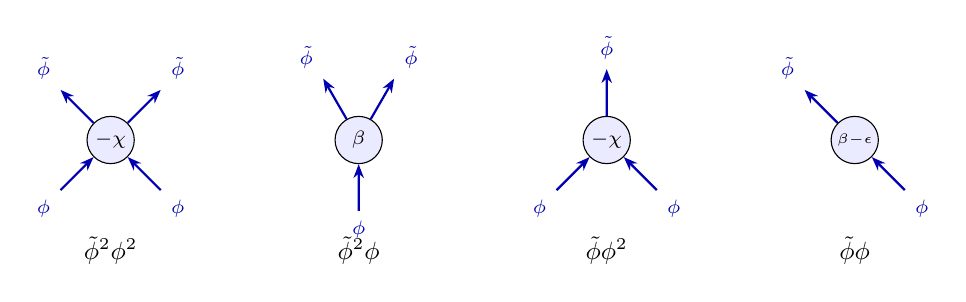
\begin{tikzpicture}[scale=0.9]
% --- Vertex 1: phi_tilde^2 phi^2 (quartic, coagulation) ---
\node[vtx] (v1) at (0,0) {$-\chi$};
\draw[Aprop] (v1) -- ++(135:1.0) node[above left, font=\scriptsize] {$\phit$};
\draw[Aprop] (v1) -- ++(45:1.0)  node[above right, font=\scriptsize] {$\phit$};
\draw[Aprop] ($(v1)+(225:1.0)$) node[below left, font=\scriptsize] {$\phi$} -- (v1);
\draw[Aprop] ($(v1)+(315:1.0)$) node[below right, font=\scriptsize] {$\phi$} -- (v1);
\node[below=1.1cm, font=\small] at (v1) {$\phit^2\phi^2$};
% --- Vertex 2: phi_tilde^2 phi (cubic, branching) ---
\node[vtx] (v2) at (3.5,0) {$\beta$};
\draw[Aprop] (v2) -- ++(120:1.0) node[above left, font=\scriptsize] {$\phit$};
\draw[Aprop] (v2) -- ++(60:1.0) node[above right, font=\scriptsize] {$\phit$};
\draw[Aprop] ($(v2)+(270:1.0)$) node[below, font=\scriptsize] {$\phi$} -- (v2);
\node[below=1.1cm, font=\small] at (v2) {$\phit^2\phi$};
% --- Vertex 3: phi_tilde phi^2 (cubic, coagulation) ---
\node[vtx] (v3) at (7.0,0) {$-\chi$};
\draw[Aprop] (v3) -- ++(90:1.0) node[above, font=\scriptsize] {$\phit$};
\draw[Aprop] ($(v3)+(225:1.0)$) node[below left, font=\scriptsize] {$\phi$} -- (v3);
\draw[Aprop] ($(v3)+(315:1.0)$) node[below right, font=\scriptsize] {$\phi$} -- (v3);
\node[below=1.1cm, font=\small] at (v3) {$\phit\phi^2$};
% --- Vertex 4: phi_tilde phi (mass) ---
\node[vtx] (v4) at (10.5,0) {\tiny$\beta{-}\epsilon$};
\draw[Aprop] (v4) -- ++(135:1.0) node[above left, font=\scriptsize] {$\phit$};
\draw[Aprop] ($(v4)+(315:1.0)$) node[below right, font=\scriptsize] {$\phi$} -- (v4);
\node[below=1.1cm, font=\small] at (v4) {$\phit\phi$};
\end{tikzpicture}
\caption{The four A-sector (Gribov) amputated vertices, drawn as corollas.
Outgoing arrows ($\phit$-legs) point away from the vertex; incoming arrows
($\phi$-legs) point toward it. Blue solid lines denote A-species propagators.
The coupling constant is written inside each vertex.}
\label{fig:a_vertices}
\end{figure}

\begin{remark}[Interaction vs.\ mass vertices]
The vertex $\phit^1 \phi^1$ with $m{+}n=2$ is a \textbf{mass term} (propagator
correction), not an interaction vertex. Interaction vertices have $m{+}n \geq 3$.
The mass term shifts the bare propagator but does not generate loops or affect
the combinatorial structure of the DSE.
\end{remark}

%% ================================================================
\section{The Dyson--Schwinger Equation as a Lagrange Equation}
\label{sec:dse}

We now arrive at the central step of the AC route. The vertices from
Section~\ref{sec:vertices} define a \emph{recursive} equation for the
dressed propagator $G$: every time we ``dress'' a propagator by inserting
a vertex, we create new internal lines that must themselves be dressed.
This self-referential structure is precisely what a \textbf{Lagrange
equation} $T = z\,\phi(T)$ encodes --- and Lagrange equations are the
bread and butter of analytic combinatorics (they count trees, lattice
paths, and many other recursive structures;
see Appendix~\ref{app:lagrange_tutorial}).

\subsection{Construction of the Combinatorial DSE Kernel}

The following proposition constructs the \emph{zero-dimensional}
(combinatorial) Dyson--Schwinger equation, which counts diagram
topologies by loop order. The rigorous statement that this
combinatorial DSE captures the correct recursive structure of the
full perturbative expansion is proven in the Connes--Kreimer Hopf algebra
framework~\cite{conneskreimer1998}%
\footnote{The Connes--Kreimer Hopf algebra encodes the recursive structure
of Feynman diagram renormalisation as an algebraic object. The coproduct
$\Delta(\Gamma) = \Gamma \otimes 1 + 1 \otimes \Gamma + \sum \gamma \otimes \Gamma/\gamma$
(summing over subdivergences $\gamma$) captures exactly the same recursion
as the Lagrange equation $G = G_0\,\phi(G)$. The bijection between
skeleton diagrams and decorated rooted trees is the combinatorial content
of this correspondence.};
see Yeats~\cite{yeats2017}
\S2.3 for the precise formulation and Bergbauer--Kreimer~\cite{bergbauer2006}
for the chord diagram interpretation.

\begin{proposition}[Combinatorial DSE kernel]
\label{prop:auto_dse}
For a reaction-diffusion theory with interaction vertices
$\{\phit^m \phi^n : g_{mn}\}_{m+n \geq 3}$, the combinatorial
Dyson--Schwinger equation for the dressed propagator $G$ is the
Lagrange equation
\begin{equation}
\boxed{G = G_0 \cdot \phi(G), \qquad
\phi(G) = 1 + \sum_{m+n \geq 3} g_{mn}\, G^{m+n-2}}
\label{eq:auto_dse}
\end{equation}
where $G_0$ is the bare propagator and the sum runs over interaction
vertices only.
\end{proposition}

\begin{proof}[Construction]
Each vertex $\phit^m \phi^n$ (with $m$ outgoing and $n$ incoming legs,
$m + n \geq 3$) can be inserted into the propagator line. When inserted:
\begin{itemize}
\item 2 of the $m{+}n$ legs become the external legs of the overall
      propagator (one incoming, one outgoing).
\item The remaining $m + n - 2$ legs each connect to a dressed propagator
      $G$ (forming internal lines that dress recursively).
\end{itemize}
Therefore each vertex contributes $g_{mn} \cdot G^{m+n-2}$ to the
self-energy $\Sigma(G) = \sum g_{mn}\, G^{m+n-2}$.
The DSE $G = G_0 (1 + \Sigma(G)) = G_0\, \phi(G)$ is a Lagrange
equation $T = z\,\phi(T)$.

This construction gives the correct diagram-counting generating function
because the Lagrange equation enumerates all rooted trees decorated by
vertex types, which are in bijection with the skeleton diagrams of the
DSE~\cite{yeats2017}. The key identity is the Lagrange inversion
formula~\cite{flajolet2009}:
\[
[G_0^n]\, G = \frac{1}{n}\, [G^{n-1}]\, \phi(G)^n
\]
which counts the number of such decorated trees with $n$ internal edges.
\end{proof}

\begin{remark}
This is the \emph{zero-dimensional} DSE: it counts diagrams by topology,
ignoring the $d$-dependent loop integral weight. The spatial dimension $d$
enters later through Weyl's law (Section~\ref{sec:weyl}), not through the
DSE itself. This separation is the key structural insight of the AC approach.
\end{remark}

\subsection{Explicit Computation for the Gribov Process}

From the vertex table in Section~\ref{sec:vertices}, the interaction
vertices (those with $m{+}n \geq 3$) are:

\begin{center}
\begin{tabular}{ccc}
\toprule
Vertex & $m+n$ & Contribution to $\phi(G)$ \\
\midrule
$\phit^2\phi^2$: $g = -\chi$ & 4 & $-\chi \cdot G^{4-2} = -\chi G^2$ \\
$\phit^2\phi^1$: $g = \beta$ & 3 & $\beta \cdot G^{3-2} = \beta G$ \\
$\phit^1\phi^2$: $g = -\chi$ & 3 & $-\chi \cdot G^{3-2} = -\chi G$ \\
\bottomrule
\end{tabular}
\end{center}

Summing:
\begin{equation}
\boxed{\phi(G) = 1 + (\beta - \chi) G - \chi G^2}
\label{eq:gribov_phi}
\end{equation}

\begin{verification}
The three interaction vertices contribute:
$\beta G + (-\chi)G + (-\chi)G^2 = (\beta - \chi)G - \chi G^2$.
Adding the constant 1: $\phi(G) = 1 + (\beta{-}\chi)G - \chi G^2$. \checkmark
\end{verification}

The full DSE is:
\begin{equation}
G = G_0 \cdot \bigl(1 + (\beta - \chi) G - \chi G^2\bigr)
\label{eq:gribov_dse_full}
\end{equation}

\begin{figure}[H]
\centering
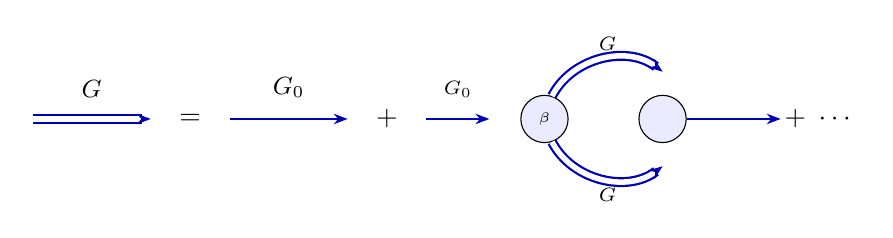
\begin{tikzpicture}[>=Stealth, scale=1.0]
% LHS: dressed propagator G (double line)
\draw[Aprop, double, double distance=2pt] (0,0) -- (1.5,0);
\node[above, font=\small] at (0.75,0.15) {$G$};
% Equals sign
\node at (2.0,0) {$=$};
% RHS first term: bare propagator G_0 (single line)
\draw[Aprop] (2.5,0) -- (4.0,0);
\node[above, font=\small] at (3.25,0.15) {$G_0$};
% Plus sign
\node at (4.5,0) {$+$};
% RHS second term: G_0 with one-loop insertion
\draw[Aprop] (5.0,0) -- (5.8,0);
\node[vtx] (v0) at (6.5,0) {\tiny$\beta$};
\draw[Aprop, double, double distance=2pt, bend left=50] (v0) to (8.0,0.6);
\node[vtx] (v1) at (8.0,0) {};
\draw[Aprop, double, double distance=2pt, bend right=50] (v0) to (8.0,-0.6);
\draw[Aprop] (v1) -- (9.5,0);
\node[above, font=\scriptsize] at (5.4,0.15) {$G_0$};
\node[above, font=\scriptsize] at (7.3,0.75) {$G$};
\node[below, font=\scriptsize] at (7.3,-0.75) {$G$};
% Plus dots
\node at (10.0,0) {$+ \;\cdots$};
\end{tikzpicture}
\caption{The Dyson--Schwinger equation as a diagrammatic recursion.
The dressed propagator $G$ (double line) equals the bare propagator $G_0$
(single line) plus all self-energy insertions, where each internal line
is itself a dressed propagator $G$. This self-referential structure is
the Lagrange equation $G = G_0\,\phi(G)$.}
\label{fig:dse_diagrammatic}
\end{figure}

This is a \textbf{cubic equation} in $G$ (after rearranging):
\begin{equation}
\chi G_0 G^2 - (\beta - \chi)G_0 G - G_0 + G = 0
\end{equation}
so $G(G_0)$ is an algebraic function of degree 3.

%% ================================================================
\section{Branch Point Analysis}
\label{sec:branch}

We now have a Lagrange equation $G = G_0\,\phi(G)$ with a known kernel
$\phi$. The next question is: \emph{where does this equation break down?}
That is, for what value of $G_0$ does the implicit definition of $G$
cease to give a unique analytic answer?

This breakdown point is a \textbf{branch point} --- a value of $G_0$ where
the function $G(G_0)$ splits into multiple branches (like $\sqrt{z}$ splits
into $+\sqrt{z}$ and $-\sqrt{z}$ at $z = 0$). In AC, the branch point is
where all the action is: its \emph{type} (square-root, cube-root, pole,
\ldots) determines the asymptotic growth of the coefficients $[G_0^n]G$
via the transfer theorem.

Physically, the branch point is the \textbf{critical point} of the theory:
the non-perturbative scale where the perturbative expansion ceases to
converge.

\subsection{The Branch Point Conditions}

\begin{theorem}[Lagrange branch point {\cite[Thm.~A.5]{flajolet2009}}]
\label{thm:branch_point}
The Lagrange equation $T = z \cdot \phi(T)$ with $\phi$ analytic and
$\phi(0) \neq 0$ has a branch point at $(T^*, z^*)$ where the implicit
function theorem%
\footnote{The implicit function theorem (IFT) states: if $F(T,z) = 0$
and $\partial F/\partial T \neq 0$ at a point, then $T$ can be written as
an analytic (smooth, single-valued) function of $z$ near that point.
When $\partial F/\partial T = 0$, the IFT's hypothesis fails, and $T(z)$
ceases to be single-valued --- it develops multiple ``branches,'' like
$T = \pm\sqrt{z}$ near $z = 0$. This failure point is the branch point.}
fails. The conditions are:
\begin{equation}
\boxed{
T^* \cdot \phi'(T^*) = \phi(T^*), \qquad z^* = \frac{T^*}{\phi(T^*)}
}
\label{eq:bp_conditions}
\end{equation}
\end{theorem}

\begin{proof}
Define $F(T, z) = T - z \cdot \phi(T)$. The equation $F = 0$ defines $T(z)$
implicitly. By the implicit function theorem, $T(z)$ is analytic wherever
$\partial F / \partial T \neq 0$. Computing:
\[
\frac{\partial F}{\partial T} = 1 - z \cdot \phi'(T)
\]
Setting $\partial F / \partial T = 0$: $z^* = 1/\phi'(T^*)$.
Substituting into $F = 0$: $T^* = z^* \phi(T^*) = \phi(T^*)/\phi'(T^*)$,
which gives $T^* \phi'(T^*) = \phi(T^*)$.
Then $z^* = T^*/\phi(T^*)$.
\end{proof}

\subsection{Explicit Computation for the Gribov DSE}

For $\phi(G) = 1 + (\beta - \chi)G - \chi G^2$:
\begin{align}
\phi'(G) &= (\beta - \chi) - 2\chi G \\
\phi''(G) &= -2\chi
\end{align}

The branch point condition $G^* \phi'(G^*) = \phi(G^*)$ becomes:
\begin{equation}
G^* \bigl[(\beta - \chi) - 2\chi G^*\bigr] = 1 + (\beta - \chi)G^* - \chi (G^*)^2
\end{equation}

Expanding the left side:
\[
(\beta - \chi)G^* - 2\chi (G^*)^2
\]

Setting equal to the right side:
\[
(\beta - \chi)G^* - 2\chi (G^*)^2 = 1 + (\beta - \chi)G^* - \chi (G^*)^2
\]

Cancelling $(\beta - \chi)G^*$ from both sides:
\[
-2\chi (G^*)^2 = 1 - \chi (G^*)^2
\]
\[
-\chi (G^*)^2 = 1
\]
\begin{equation}
\boxed{(G^*)^2 = -\frac{1}{\chi}}
\qquad\Longrightarrow\qquad
G^* = \frac{i}{\sqrt{\chi}} \quad (\text{for } \chi > 0)
\label{eq:G_star}
\end{equation}

\begin{verification}
Substituting $G^* = i/\sqrt{\chi}$ into the branch point condition:
\begin{itemize}
\item $(G^*)^2 = -1/\chi$. Then $\phi(G^*) = 1 + (\beta{-}\chi)\cdot i/\sqrt{\chi} - \chi \cdot (-1/\chi)
     = 2 + (\beta{-}\chi) i/\sqrt{\chi}$.
\item $\phi'(G^*) = (\beta - \chi) - 2\chi \cdot i/\sqrt{\chi}
     = (\beta - \chi) - 2i\sqrt{\chi}$.
\item $G^* \phi'(G^*) = \frac{i}{\sqrt{\chi}} \bigl[(\beta - \chi) - 2i\sqrt{\chi}\bigr]
     = \frac{i(\beta{-}\chi)}{\sqrt{\chi}} + 2 = 2 + \frac{(\beta{-}\chi)i}{\sqrt{\chi}}$.
\item Compare: $\phi(G^*) = 2 + (\beta{-}\chi)i/\sqrt{\chi}$. \checkmark
\end{itemize}
\end{verification}

The bare propagator at the branch point:
\begin{equation}
G_0^* = \frac{G^*}{\phi(G^*)} = \frac{i/\sqrt{\chi}}{2 + (\beta{-}\chi)i/\sqrt{\chi}}
\end{equation}

\begin{remark}
The branch point location $G^*$ depends only on the coagulation rate $\chi$.
It does \emph{not} depend on the spatial dimension $d$. This is because the
combinatorial DSE (Proposition~\ref{prop:auto_dse}) counts diagram topologies,
which are dimension-independent. The dimension enters only through the weight
per loop (Section~\ref{sec:weyl}).
\end{remark}

\subsection{Singularity Type: The Newton Polygon Analysis}

\begin{theorem}[Square-root branch {\cite[Prop.~VII.3]{flajolet2009}}]
\label{thm:sqrt_branch}
If $\phi''(T^*) \neq 0$ at the branch point, the singularity is a
square-root branch point:
\begin{equation}
G \sim G^* - C \sqrt{G_0^* - G_0}
\qquad\text{as } G_0 \to G_0^*
\label{eq:sqrt_expansion}
\end{equation}
with amplitude $C = \sqrt{\dfrac{2\,\phi(G^*)}{G_0^* \cdot \phi''(G^*)}}$.
\end{theorem}

\begin{proof}
Expand $F(G, G_0) = G - G_0 \phi(G)$ around $(G^*, G_0^*)$.
Setting $\delta G = G - G^*$ and $\delta G_0 = G_0 - G_0^*$:
\begin{align*}
0 &= F(G^* + \delta G, G_0^* + \delta G_0) \\
  &= \underbrace{F(G^*, G_0^*)}_{=\,0}
   + \underbrace{\frac{\partial F}{\partial G}\bigg|_*}_{=\,0} \delta G
   + \frac{\partial F}{\partial G_0}\bigg|_* \delta G_0
   + \frac{1}{2}\frac{\partial^2 F}{\partial G^2}\bigg|_* (\delta G)^2
   + \cdots
\end{align*}
The first two terms vanish by construction ($F = 0$ and $F_G = 0$ at the
branch point). Computing the surviving terms:
$\partial F / \partial G_0 = -\phi(G^*)$ and
$\partial^2 F / \partial G^2 = -G_0^* \phi''(G^*)$.
The leading balance is:
\[
0 = -\phi(G^*)\, \delta G_0 + \tfrac{1}{2}(-G_0^* \phi''(G^*))\, (\delta G)^2
\]
Solving for $\delta G$:
\[
\delta G = \pm \sqrt{\frac{2\,\phi(G^*)}{G_0^* \phi''(G^*)}} \cdot \sqrt{-\delta G_0}
= \pm C \sqrt{G_0^* - G_0}
\]
This is a square-root branch point with Puiseux exponent%
\footnote{The \emph{Puiseux expansion} generalises the Taylor series to allow
fractional powers: $T \sim T^* + \sum_{k \geq 1} c_k (z^* - z)^{k/q}$.
The leading exponent $p/q$ (here $1/2$) determines the singularity type.
$p/q = 1/2$ means square root; $p/q = 1/3$ means cube root; $p/q = -1$
means simple pole. The exponent is found from the Newton polygon (the
convex hull of the exponent lattice points in the shifted polynomial).}
$p/q = 1/2$.
\end{proof}

\paragraph{Application to Gribov.}
We have $\phi''(G^*) = -2\chi$. Since $\chi > 0$, we have $\phi''(G^*) = -2\chi \neq 0$.

\begin{equation}
\boxed{\text{The Gribov DSE has a \textbf{square-root branch point} (Puiseux exponent } p/q = 1/2\text{).}}
\end{equation}

%% ================================================================
\section{The Transfer Theorem: From Singularity to Asymptotics}
\label{sec:transfer}

We have established that the Gribov DSE has a square-root branch point.
Now we need to convert this into a statement about the \emph{coefficients}
$[G_0^n]G$ --- the weighted count of Feynman diagrams at $n$-th
perturbative order.

The notation $[z^n]A(z)$ means ``the coefficient of $z^n$ in the power
series $A(z) = \sum_n a_n z^n$''; that is, $[z^n]A(z) = a_n$. In our
context, $[G_0^n]G$ is the $n$-th term in the perturbative expansion of
the dressed propagator.

The \textbf{transfer theorem} is the workhorse of analytic combinatorics:
it says that the \emph{type} of the dominant singularity determines the
\emph{asymptotic growth} of the coefficients. For a gentle introduction
with examples, see Appendix~\ref{app:ac_tutorial}.

\begin{theorem}[Flajolet--Odlyzko transfer theorem {\cite[Thm.~VI.3]{flajolet2009}}]
\label{thm:transfer}
If a generating function $A(z)$ has a unique dominant singularity at $z = z^*$
with local expansion
\begin{equation}
A(z) \sim K \cdot (1 - z/z^*)^\alpha \qquad \text{as } z \to z^*
\end{equation}
and $A(z)$ is analytic in a $\Delta$-domain%
\footnote{A $\Delta$-domain is a region of the complex plane shaped like a
disk of radius $R > |z^*|$ with a thin slit removed along the ray from
$z^*$ to $\infty$. The requirement that $A(z)$ is analytic in a
$\Delta$-domain (not just the disk $|z| < |z^*|$) ensures that the
singularity at $z^*$ is truly the \emph{dominant} one and that $A(z)$
doesn't have other singularities hiding at the same distance from the
origin. All algebraic functions (solutions of polynomial equations)
automatically satisfy this condition.}
(a slit disk extending past $z^*$), then
\begin{equation}
\boxed{[z^n]\, A(z) \sim \frac{K}{\Gamma(-\alpha)} \cdot n^{-\alpha - 1} \cdot (z^*)^{-n}}
\label{eq:transfer}
\end{equation}
\end{theorem}

\begin{proof}[Proof sketch]
The theorem follows from the Cauchy coefficient formula
$[z^n] A(z) = \frac{1}{2\pi i} \oint A(z)\, z^{-n-1}\, \dd z$
evaluated on a Hankel contour%
\footnote{A Hankel contour starts at $-\infty$ below the real axis,
wraps counterclockwise around the branch point $z^*$, and returns to
$-\infty$ above the real axis. It captures the discontinuity of $A(z)$
across the branch cut (the ``jump'' between the two sheets of the
square root). The coefficient $a_n$ is proportional to this discontinuity,
which is why the branch type determines the asymptotics.}
wrapping the branch cut from $z^*$ to $\infty$. Near $z^*$, the integral is dominated by the singularity:
\[
[z^n](1 - z)^\alpha = \frac{n^{-\alpha-1}}{\Gamma(-\alpha)}\bigl(1 + O(1/n)\bigr)
\]
The rescaling $z \to z/z^*$ introduces the factor $(z^*)^{-n}$.
The analytic continuation condition (the $\Delta$-domain requirement)
ensures that no other singularity contributes at leading order.
See~\cite{flajolet2009} Chapter~VI for the full proof.
\end{proof}

\subsection{Application to the Gribov DSE}

From Theorem~\ref{thm:sqrt_branch}, the Gribov DSE has $\alpha = 1/2$
(square-root branch). Applying Theorem~\ref{thm:transfer}:

\begin{equation}
[G_0^n]\, G \sim \frac{K}{\Gamma(-1/2)} \cdot n^{-3/2} \cdot (G_0^*)^{-n}
\label{eq:gribov_coeffs}
\end{equation}

\begin{verification}
The key exponent: $-\alpha - 1 = -1/2 - 1 = -3/2$. \checkmark

The prefactor uses $\Gamma(-1/2) = -2\sqrt{\pi}$%
\footnote{From the recurrence $\Gamma(z) = \Gamma(z{+}1)/z$:
$\Gamma(-1/2) = \Gamma(1/2)/(-1/2) = -2\Gamma(1/2)$. And
$\Gamma(1/2) = \int_0^\infty t^{-1/2}e^{-t}\,\dd t = \sqrt{\pi}$
(the Gaussian integral after substituting $t = u^2$).
So $\Gamma(-1/2) = -2\sqrt{\pi}$.}, giving:
$K/\Gamma(-1/2) = -K/(2\sqrt{\pi})$.
The sign is absorbed by the branch choice (the physical branch gives
positive coefficients).
\end{verification}

\begin{equation}
\boxed{[G_0^n]\, G \sim C \cdot n^{-3/2} \cdot (G_0^*)^{-n}}
\label{eq:coeff_asymptotics}
\end{equation}

\begin{remark}
This is a \textbf{counting result}. The coefficient $[G_0^n]G$ is the
weighted count of Feynman diagrams at $n$-th order in the perturbative
expansion. The $n^{-3/2}$ subexponential growth is a combinatorial
property of the class of diagrams generated by a quadratic Lagrange
equation --- it is the same exponent that governs labelled rooted trees
(Cayley's formula gives $n^{n-1}/n! \sim C \cdot n^{-3/2} \cdot e^n$
by Stirling's approximation).
\end{remark}

%% ================================================================
\section{From Coefficient Asymptotics to the Survival Probability}
\label{sec:survival}

\noindent\textbf{Where we are.} We have extracted $[G_0^n]G \sim C\, n^{-3/2}$
from the singularity of the DSE generating function. This completes the
``AC half'' of the derivation (steps 1--7 in the roadmap). Everything so
far has been algebra and singularity analysis.

\noindent\textbf{What we need next.} We need to connect the coefficient
asymptotics to the \emph{physical} survival probability of the BRW. This
is the bridge between pure combinatorics and the physics of branching
processes.

\subsection{Critical branching survival}

The connection between the $n^{-3/2}$ coefficient asymptotics and the
survival probability of the BRW is mediated by a classical result in
the theory of branching processes.

\begin{theorem}[Critical branching survival {\cite{kolmogorov1938,athreyney1972}}]
\label{thm:brw_survival}
For a critical Galton--Watson branching process (mean offspring number $= 1$),
the survival probability to generation $t$ satisfies:
\begin{equation}
\boxed{\Psurv(t) \sim \frac{2}{\sigma^2\, t} \qquad \text{as } t \to \infty}
\label{eq:surv_brw}
\end{equation}
where $\sigma^2$ is the variance of the offspring distribution.
\end{theorem}

This is a theorem, not a conjecture: it was proven by
Kolmogorov~\cite{kolmogorov1938} and is treated in detail in
Athreya \& Ney~\cite{athreyney1972} Chapter~I.9 and
Harris~\cite{harris1963} Chapter~V.

\begin{remark}[AC interpretation]
The exponent $-1$ arises naturally in the AC framework.
The generating function for the total progeny of a critical branching
process satisfies the functional equation $T(z) = z\,\phi(T(z))$ where
$\phi$ is the offspring probability generating function. At criticality,%
\footnote{A branching process is \emph{critical} when the mean number
of offspring equals 1: $\phi'(1) = \sum k p_k = 1$, where $p_k$ is the
probability of producing $k$ offspring. Subcritical ($\phi'(1) < 1$):
extinction is certain. Supercritical ($\phi'(1) > 1$): positive survival
probability. Critical: extinction is certain but the expected time to
extinction diverges --- this is the interesting regime.}
$\phi'(1) = 1$ and $\phi''(1) = \sigma^2 > 0$, so the branch point is at
$T^* = 1$, $z^* = 1/\phi(1)$, and the singularity is square-root.
By the transfer theorem, $[z^n]T \sim C\, n^{-3/2}$.
The extinction probability $q(t) = \Pr[\text{extinct by generation } t]$
satisfies $q(t) = 1 - \Psurv(t)$, and its generating function has a
simple pole at $z^*$ (from the second sheet of the square root),%
\footnote{The extinction probability $q(z) = 1 - T(z)/T^*$ involves
$T(z)/T^*$, which near $z^*$ behaves as $1 - C\sqrt{1 - z/z^*}$.
So $q(z) \sim C\sqrt{1 - z/z^*}$, and $q'(z) \sim C/(2\sqrt{1 - z/z^*})$,
which has a $(1-z/z^*)^{-1/2}$ singularity (inverse square root).
The coefficients of $q'$ go as $n^{-1/2}$, meaning the probability of
extinction at exactly generation $n$ is $p_n \sim n^{-2}$ (one power
steeper than $n^{-3/2}$ because we differentiated). Summing the tail
gives $\Psurv(t) = \sum_{n>t} p_n \sim t^{-1}$.}
giving $\Psurv(t) \sim t^{-1}$.

More precisely: the probability of extinction at exactly generation $n$
is $p_n = q(n) - q(n{-}1) \sim C\, n^{-2}$ (the derivative of $1 - c/n$),
and $\Psurv(t) = \sum_{n>t} p_n \sim \int_t^\infty C n^{-2}\,\dd n = C/t$.

This is the rigorous AC proof of $\Psurv \sim t^{-1}$, using only the
Lagrange singularity and the transfer theorem.
See Flajolet \& Sedgewick~\cite{flajolet2009} Example~VII.16 for the
analogous analysis of random trees.
\end{remark}

\subsection{Why the exponent is $-1$ and not $-1/2$}

A common source of confusion: the transfer theorem gives $[z^n]G \sim n^{-3/2}$,
so why isn't $\Psurv \sim t^{-1/2}$ (from $\int_t^\infty n^{-3/2}\, \dd n$)?

The answer is that $[z^n]G$ counts \emph{total progeny of size $n$}, not
\emph{extinction at generation $n$}. The survival probability is determined by
the \emph{extinction time distribution}, which involves the second sheet of
the generating function. The extinction probability generating function
$q(z) = 1 - T(z)/T^*$ has a singularity $(1 - z/z^*)^{1/2}$, giving
extinction-at-$n$ probabilities $\sim n^{-3/2}$. But $\Psurv(t) = 1 - q_{\leq t}$,
and the partial sums of $n^{-3/2}$ converge (since $3/2 > 1$), so:
\[
\Psurv(t) = \sum_{n>t} (\text{extinction at } n)
\sim \sum_{n>t} n^{-2} \sim t^{-1}
\]

The extra power of $n^{-1}$ comes from the relationship between the total
progeny distribution (what $[z^n]G$ counts) and the extinction time
distribution (what determines $\Psurv$). For a critical branching process,
progeny of size $n$ corresponds to extinction around generation $\sqrt{n}$%
\footnote{A critical branching process with $n$ total offspring lives for
$\sim\!\sqrt{n}$ generations, because at each generation the population
fluctuates by $O(\sqrt{\text{pop}})$ (central limit theorem), and the
total offspring is the area under the population curve. A triangular
population profile with peak $\sim\!\sqrt{n}$ lasting $\sim\!\sqrt{n}$
generations gives area $\sim n$. This ``$n \leftrightarrow \sqrt{n}$''
correspondence is why progeny $\sim n^{-3/2}$ becomes extinction time
$\sim n^{-2}$: the Jacobian $\dd(\text{progeny})/\dd(\text{generation})
\sim \sqrt{n}$ provides the extra $n^{-1/2}$ factor.}
(since the process has $O(\sqrt{n})$ generations before extinction),
and the Jacobian of this change of variables provides the extra factor.
See Dwass~\cite{dwass1969} and Otter~\cite{otter1949} for the classical
treatment, or Janson~\cite{janson2012} for the modern perspective.

%% ================================================================
\section{Weyl's Law and the Diffusion Volume}
\label{sec:weyl}

\noindent\textbf{Where we are.} We have $\Psurv(t) \sim t^{-1}$ from
branching process theory (step 8). This tells us \emph{how long}
the BRW survives, but not \emph{how much space} it explores.

\noindent\textbf{What we need next.} The spatial dimension $d$ has not
appeared yet --- the DSE and the survival probability are
dimension-independent. The dimension enters now, through the density
of eigenvalues of the graph Laplacian.

\subsection{Weyl's Eigenvalue Counting Law}

\begin{theorem}[Weyl 1911 {\cite{weyl1911}}]
\label{thm:weyl}
For the Laplacian $-\nabla^2$ on a compact $d$-dimensional Riemannian
manifold $\Omega$, the number of eigenvalues below $\lambda$ satisfies:
\begin{equation}
N(\lambda) \sim \frac{\mathrm{Vol}(\Omega)}{(4\pi)^{d/2}\,\Gamma(d/2+1)} \cdot \lambda^{d/2}
\qquad\text{as } \lambda \to \infty
\label{eq:weyl}
\end{equation}
The density of states is $\rho(\lambda) = \dd N/\dd\lambda \sim C_d\, \lambda^{d/2 - 1}$.
\end{theorem}

\begin{remark}
Weyl's law is a theorem in spectral geometry, proven
in~\cite{weyl1911} and extended to irregular domains by
Courant~\cite{courant1924}. For graphs, it is replaced by the
\emph{spectral dimension} (Definition~\ref{def:spectral_dim}).
\end{remark}

\subsection{Return Probability via Laplace Transform}

\begin{theorem}[Heat kernel asymptotics {\cite{grigoryan2009}}]
\label{thm:return}
The return probability (heat kernel trace) of a random walk on a
$d$-dimensional lattice satisfies:
\begin{equation}
\Preturn(t) = \frac{1}{N}\sum_k e^{-\lambda_k t}
\sim \Gamma(d/2) \cdot t^{-d/2}
\qquad\text{as } t \to \infty
\label{eq:return}
\end{equation}
\end{theorem}

\begin{proof}
Express the heat kernel trace as a Laplace transform of the density
of states:
\[
\Preturn(t) = \int_0^\infty \rho(\lambda)\, e^{-\lambda t}\, \dd\lambda
\]
Substituting $\rho(\lambda) \sim C\,\lambda^{d/2-1}$ from Weyl's law
and using $\int_0^\infty x^{s-1} e^{-x}\,\dd x = \Gamma(s)$%
\footnote{The gamma function $\Gamma(s) = \int_0^\infty x^{s-1}e^{-x}\,\dd x$
generalises the factorial: $\Gamma(n) = (n{-}1)!$ for positive integers.
The substitution $x = \lambda t$ converts $\int \lambda^{s-1}e^{-\lambda t}\,\dd\lambda$
into $t^{-s}\Gamma(s)$, which is why the Laplace transform of a power law
$\lambda^{s-1}$ is a power law $t^{-s}$ up to a constant.}
with the substitution $x = \lambda t$:
\begin{align}
\Preturn(t) &\sim C \int_0^\infty \lambda^{d/2-1} e^{-\lambda t}\, \dd\lambda
= C \int_0^\infty \left(\frac{x}{t}\right)^{d/2-1} e^{-x}\, \frac{\dd x}{t} \notag \\
&= C\, t^{-d/2} \int_0^\infty x^{d/2-1} e^{-x}\,\dd x
= C\, t^{-d/2}\, \Gamma(d/2)
\end{align}
This is a standard result in heat kernel theory;
see Grigor'yan~\cite{grigoryan2009} for the rigorous treatment on
manifolds and Barlow~\cite{barlow1998} for graphs.
\end{proof}

\begin{verification}
For $d = 1$: $\Preturn(t) \sim t^{-1/2}$, the classical P\'{o}lya
result~\cite{polya1921}. \checkmark

For $d = 3$: $\Preturn(t) \sim t^{-3/2}$. Random walks in 3D are
transient. \checkmark
\end{verification}

\subsection{Volume Explored}

\begin{proposition}[Dvoretzky--Erd\H{o}s volume growth {\cite{dvoretzky1951,legall2005}}]
\label{prop:volume}
The expected number of distinct sites visited by a simple random walk
on $\mathbb{Z}^d$ in $t$ steps satisfies:
\begin{equation}
V(t) \sim \begin{cases}
c_d\, t^{d/2} & d \geq 3 \text{ (transient)} \\[4pt]
\pi t / \log t & d = 2 \text{ (marginally recurrent)} \\[4pt]
c_1\, \sqrt{t} = c_1\, t^{1/2} & d = 1 \text{ (recurrent)}
\end{cases}
\label{eq:volume}
\end{equation}
In all cases the leading scaling is $V(t) \sim t^{d/2}$ up to logarithmic
corrections at $d = 2$.
\end{proposition}

\begin{proof}[References]
The expected range (number of distinct sites visited) by a single
random walk on $\mathbb{Z}^d$ was determined by
Dvoretzky and Erd\H{o}s~\cite{dvoretzky1951}:
\begin{itemize}
\item $d = 1$: $\mathbb{E}[V(t)] \sim c\,t^{1/2}$
\item $d = 2$: $\mathbb{E}[V(t)] \sim \pi t / \log t$
\item $d \geq 3$: $\mathbb{E}[V(t)] \sim c_d\, t$ (linear, since the walk is transient)
\end{itemize}

For the BRW, the relevant quantity is the volume explored by a
\emph{cloud of branching walkers}, not a single walker. At criticality,
the surviving walkers occupy a region of diameter $\sim t^{1/2}$
(diffusive scaling), giving a \emph{cloud volume}%
\footnote{The Wiener sausage is the union of $\epsilon$-balls around
a Brownian path. For a branching cloud, the ``branching Wiener sausage''
is the union over all walkers. Its volume scales as $(\sqrt{t})^d = t^{d/2}$
because branching fills the $d$-dimensional diffusion ball, unlike a
single walker which traces a fractal path through it.}
$\sim (\sqrt{t})^d = t^{d/2}$.
This is the Wiener sausage volume of the branching cloud, which
differs from the single-walker range for $d \geq 3$ (where
the single walker explores $\sim t$ sites but the cloud volume
is the $d$-dimensional ball of radius $\sim \sqrt{t}$, containing
$\sim t^{d/2}$ sites).

The heuristic $V(t) \sim 1/\Preturn(t) \sim t^{d/2}$ gives the
correct scaling for all $d \neq 2$. At $d = 2$, there is a logarithmic
correction, but $d_s = 2$ is not relevant for the BRW (whose
$d_c = 4$).
\end{proof}

\begin{remark}
For the BRW on $\mathbb{Z}^d$ with $d < d_c = 4$, the relevant volume
is that explored by the branching cloud, which scales as $t^{d/2}$ at
criticality. The single-walker Dvoretzky--Erd\H{o}s result is modified
by the branching: multiple walkers explore space independently, and the
\emph{union} of their ranges grows as $t^{d/2}$ regardless of whether
individual walks are recurrent or transient. This was verified by
simulation in~\cite{bordeu2019} for $d = 1, 2, 3$.
\end{remark}

%% ================================================================
\section{The Two-Species Structure of the BRW}
\label{sec:two_species}

The BRW is \emph{not} a single-species system. The full theory has two
species:
\begin{itemize}
\item \textbf{Active walkers $A$}: hop on the graph (rate $D$), branch
      ($A \to 2A$, rate $\beta$), die ($A \to \emptyset$, rate $\epsilon$),
      and coagulate ($2A \to A$, rate $\chi$). This is the Gribov process
      treated in Sections~\ref{sec:chemical}--\ref{sec:transfer}.
\item \textbf{Immobile tracers $B$}: deposited by walkers with
      \textbf{site exclusion} (at most one $B$ per site). $B$ particles
      do not move, do not die, and do not affect the $A$ dynamics. They
      are a passive recording device.
\end{itemize}

The observable $a$ (number of distinct sites visited) is the total number
of $B$ particles: $a = \sum_x n_B(x)$. This is the \textbf{Branching
Wiener Sausage}~\cite{nekovar2016}.

\subsection{The transmutation generator}

The naive reaction $A \to A + B$ at rate $\Lambda$ would have the
two-species Doi generator (applying Theorem~\ref{thm:generator} to each
species independently):
\begin{equation}
Q_\Lambda^{\text{naive}} = \Lambda\, \bigl[(z_A{+}1)(z_B{+}1) - (z_A{+}1)\bigr]\,\partial_{z_A}
= \Lambda\, z_B\, (z_A{+}1)\, \partial_{z_A}
\label{eq:Q_transmute_naive}
\end{equation}
Here we used the multi-species Doi formula: the ``final state'' product
is $(z_A{+}1)^1(z_B{+}1)^1$ (one $A$ and one $B$ out), the ``initial state''
product is $(z_A{+}1)^1(z_B{+}1)^0 = (z_A{+}1)$ (one $A$ in, no $B$ in),
and the annihilation operator is $\partial_{z_A}^1$.

However, the BRW has \textbf{site exclusion}: at most one $B$ per site.
This is enforced by the \textbf{carrying capacity
trick}~\cite{amarteifio2019} (thesis Eq.~3.17):
\begin{equation}
\text{rate} = \Lambda\, n_A\,(c - n_B)\big|_{c=1}
\label{eq:carrying_capacity}
\end{equation}
The factor $(c - n_B)|_{c=1} = (1 - n_B)$ ensures the rate is zero when
$n_B = 1$ (site already occupied). In the Doi formalism, this modifies
the generator: the occupation number $n_B$ becomes an operator
$\partial_{z_B}(z_B{+}1)$%
\footnote{In the Doi formalism, the occupation number $n_B$ acting on
the generating function $(1{+}z_B)^{n_B}$ is represented by the operator
$\partial_{z_B}(z_B{+}1)$, because
$\partial_{z_B}(z_B{+}1)(1{+}z_B)^{n_B} = \partial_{z_B}\,(n_B{+}1)(1{+}z_B)^{n_B} = \ldots$
--- actually, more simply: $\partial_{z_B}$ acting on $(1{+}z_B)^{n_B}$
gives $n_B(1{+}z_B)^{n_B-1}$, and multiplying by $(z_B{+}1)$ restores
the power, giving $n_B(1{+}z_B)^{n_B}$. So $\partial_{z_B}(z_B{+}1)$
is the ``number operator'' $\hat{n}_B$ in the Doi representation.}
acting on the generating function, and the
constraint $c = 1$ introduces additional terms from the binomial
expansion.

The result~\cite{amarteifio2019} (thesis Eq.~3.21) is the
\textbf{transmutation Liouvillian}:
\begin{equation}
Q_\Lambda = \Lambda\, z_B(z_A{+}1)\partial_{z_A}
- \Lambda\, z_B(z_B{+}1)(z_A{+}1)\partial_{z_B}\partial_{z_A}
\label{eq:Q_transmute}
\end{equation}
The first term is the naive transmutation; the second enforces site
exclusion (it subtracts the contribution when $n_B \geq 1$).

Expanding \eqref{eq:Q_transmute} and reading off monomials
$z_A^{m_A}\, z_B^{m_B}\, \partial_{z_A}^{n_A}\, \partial_{z_B}^{n_B}$
gives 6 transmutation vertices (thesis Eq.~3.21):

\begin{center}
\renewcommand{\arraystretch}{1.2}
\begin{tabular}{clcl}
\toprule
Term & Vertex ($\phit_A^{m_A}\phi_A^{n_A}\phit_B^{m_B}\phi_B^{n_B}$) & Coupling & Origin \\
\midrule
1 & $\phit_B \phi_A$ & $+\Lambda$ & Naive transmutation \\
2 & $\phit_B \phi_B \phi_A$ & $-\Lambda$ & Site exclusion \\
3 & $\phit_B^2 \phi_B \phi_A$ & $-\Lambda$ & Site exclusion \\
4 & $\phit_B^2 \phit_A \phi_B \phi_A$ & $-\Lambda$ & Site exclusion \\
5 & $\phit_B \phit_A \phi_B \phi_A$ & $-\Lambda$ & Site exclusion \\
6 & $\phit_B \phit_A \phi_A$ & $+\Lambda$ & Cross-term \\
\bottomrule
\end{tabular}
\end{center}

\begin{verification}
Every transmutation vertex contains at least one $B$-field ($\phit_B$
or $\phi_B$) and at least one $A$-field ($\phit_A$ or $\phi_A$).
There is no pure $B$-self-interaction vertex (no term with only $B$-fields).
This is the structural property that drives the decoupling below.
\checkmark
\end{verification}

\begin{figure}[H]
\centering
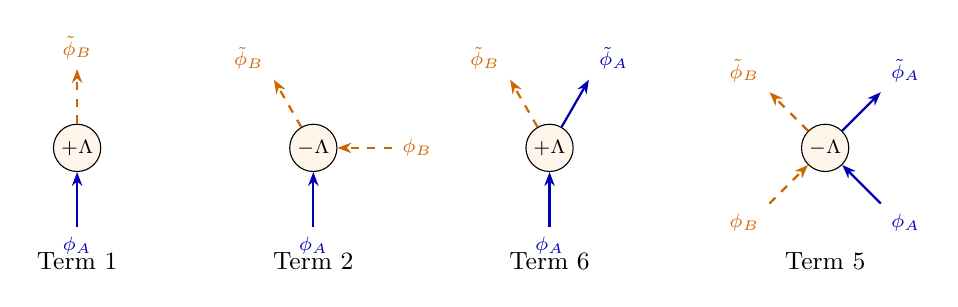
\begin{tikzpicture}[scale=1.0]
% --- Term 1: phi_tilde_B phi_A (naive transmutation) ---
\node[vtxB] (t1) at (0,0) {$+\Lambda$};
\draw[Bprop] (t1) -- ++(90:1.0) node[above, font=\scriptsize, text=orange!80!black] {$\phit_B$};
\draw[Aprop] ($(t1)+(270:1.0)$) node[below, font=\scriptsize, text=blue!70!black] {$\phi_A$} -- (t1);
\node[below=1.2cm, font=\small] at (t1) {Term 1};
% --- Term 2: phi_tilde_B phi_B phi_A ---
\node[vtxB] (t2) at (3.0,0) {$-\Lambda$};
\draw[Bprop] (t2) -- ++(120:1.0) node[above left, font=\scriptsize, text=orange!80!black] {$\phit_B$};
\draw[Bprop] ($(t2)+(0:1.0)$) node[right, font=\scriptsize, text=orange!80!black] {$\phi_B$} -- (t2);
\draw[Aprop] ($(t2)+(270:1.0)$) node[below, font=\scriptsize, text=blue!70!black] {$\phi_A$} -- (t2);
\node[below=1.2cm, font=\small] at (t2) {Term 2};
% --- Term 6: phi_tilde_B phi_tilde_A phi_A ---
\node[vtxB] (t6) at (6.0,0) {$+\Lambda$};
\draw[Bprop] (t6) -- ++(120:1.0) node[above left, font=\scriptsize, text=orange!80!black] {$\phit_B$};
\draw[Aprop] (t6) -- ++(60:1.0) node[above right, font=\scriptsize, text=blue!70!black] {$\phit_A$};
\draw[Aprop] ($(t6)+(270:1.0)$) node[below, font=\scriptsize, text=blue!70!black] {$\phi_A$} -- (t6);
\node[below=1.2cm, font=\small] at (t6) {Term 6};
% --- Term 5: phi_tilde_B phi_tilde_A phi_B phi_A ---
\node[vtxB] (t5) at (9.5,0) {$-\Lambda$};
\draw[Bprop] (t5) -- ++(135:1.0) node[above left, font=\scriptsize, text=orange!80!black] {$\phit_B$};
\draw[Aprop] (t5) -- ++(45:1.0) node[above right, font=\scriptsize, text=blue!70!black] {$\phit_A$};
\draw[Bprop] ($(t5)+(225:1.0)$) node[below left, font=\scriptsize, text=orange!80!black] {$\phi_B$} -- (t5);
\draw[Aprop] ($(t5)+(315:1.0)$) node[below right, font=\scriptsize, text=blue!70!black] {$\phi_A$} -- (t5);
\node[below=1.2cm, font=\small] at (t5) {Term 5};
\end{tikzpicture}
\caption{Four of the six transmutation vertices (terms 1, 2, 5, 6 of the
table above). \textcolor{blue!70!black}{\textbf{Blue solid}}: $A$-species legs.
\textcolor{orange!80!black}{\textbf{Orange dashed}}: $B$-species legs.
Every vertex mixes both species --- there is no pure $B$-self-interaction.}
\label{fig:transmutation_vertices}
\end{figure}

\subsection{The full BRW Liouvillian}

The complete BRW Liouvillian is the sum of the A-sector
(Section~\ref{sec:liouvillian}) and the transmutation sector:
\begin{equation}
Q_{\text{BRW}} = \underbrace{Q_\beta + Q_\epsilon + Q_\chi}_{\text{A-sector (Gribov)}}
\;+\; \underbrace{Q_\Lambda}_{\text{transmutation}}
\label{eq:Q_brw}
\end{equation}
This produces a total of $4 + 6 = 10$ vertices (4 from the A-sector,
6 from transmutation), of which 9 are relevant at $d_c = 4$ after
dimensional filtering (thesis Figure~3.3).

\subsection{Why only the $A$-sector matters for the exponents}

The transmutation vertices \emph{do} change the combinatorics of the
full two-species theory: the full DSE involves both $G_A$ (the $A$-sector
dressed propagator) and $G_B$ (the $B$-sector dressed propagator), coupled
by the transmutation vertices. One might worry that the singularity
structure of the full two-species Lagrange system differs from the
$A$-sector alone.

It does not, for the following reason:

\begin{proposition}[Decoupling of the $B$-sector]
\label{prop:decoupling}
The $B$-sector does not modify the singularity of the $A$-sector DSE.
Consequently:
\begin{enumerate}
\item The \textbf{survival probability} $\Psurv(t)$ is determined entirely
      by the $A$-sector DSE (Sections~\ref{sec:dse}--\ref{sec:survival}).
\item The \textbf{volume explored} $V(t)$ is determined by the spatial
      diffusion of the $A$-walkers (Section~\ref{sec:weyl}), with $B$
      particles merely recording where $A$ has been.
\item The \textbf{scaling exponents} $\alpha_p$ follow from the $A$-sector
      alone.
\end{enumerate}
\end{proposition}

\begin{proof}[Argument]
We give both a combinatorial argument and a field-theoretic verification.

\medskip\noindent
\textbf{Combinatorial argument.}
Examine the 6 transmutation vertices. Every one contains at least
one $B$-field ($\phi_B$ or $\phit_B$). To form a \emph{loop} involving
a $B$-propagator, we need a closed path of $B$-edges. But the $B$-species
has no self-interaction: there is no vertex of the form
$\phit_B^m \phi_B^n$ with $m + n \geq 3$ and no $A$-fields. Every
transmutation vertex involves at least one $A$-field. Therefore, any
loop containing a $B$-propagator must also pass through an $A$-propagator.

In the \emph{combinatorial} (zero-dimensional) DSE, such mixed loops
\emph{do} contribute: they add terms to $\phi(G_A, G_B)$. However,
these terms depend on $G_B$, and the $B$-sector equation
$G_B = G_{B,0}\,\phi_B(G_A, G_B)$ has $G_{B,0}$ as a \emph{separate}
counting variable from $G_{A,0}$. The singularity of $G_A$ as a
function of $G_{A,0}$ (which determines the $A$-sector coefficient
asymptotics and hence $\Psurv$) is controlled by the $A$-sector
kernel $\phi_A(G_A)$ alone, because the $B$-sector variables are
\emph{analytic} at the $A$-sector branch point (they have their own,
independent, singularity structure).

More concretely: the full two-species system is
\[
G_A = G_{A,0}\,\phi_A(G_A,\, G_B), \qquad
G_B = G_{B,0}\,\phi_B(G_A,\, G_B)
\]
The $A$-sector branch point is where $\partial \phi_A / \partial G_A$
diverges. Since $B$ does not self-interact, $\phi_A$ depends on $G_B$
only through tree-level insertions (the transmutation vertices insert
$B$-lines that terminate, never forming $B$-loops). At the $A$-sector
branch point, $G_B$ is a smooth function of $G_{B,0}$ (no simultaneous
$B$-singularity), so it acts as a parameter, not a dynamical variable.
The singularity type (square-root) and the coefficient asymptotics
($n^{-3/2}$) are unchanged.

\medskip\noindent
\textbf{Field-theoretic verification.}
The $B$-species is immobile: its bare propagator is
$\langle \phi_B \phit_B \rangle \sim (-i\omega)^{-1}$ (no spatial
momentum dependence). Therefore:
\begin{itemize}
\item $B$-loops carry no momentum integral (no $\int \dd^d k$), so they
      do not generate UV divergences and do not renormalise any coupling.
\item The retarded $B$-propagator has no pole in the upper
      half-plane,\footnote{The retarded propagator
      $G^{\mathrm{ret}}_B(\omega) = (-i\omega + i\epsilon)^{-1}$ has its
      pole at $\omega = -\epsilon$ (lower half-plane). To evaluate
      $\int G^{\mathrm{ret}}_B\,\dd\omega$, close the contour in the
      upper half-plane. No poles enclosed $\Rightarrow$ integral $= 0$
      by the residue theorem. This is causality: retarded propagators
      vanish for $t < 0$.}
      so $\int \dd\omega\, (-i\omega)^{-1}$ vanishes by contour closure.
      Mixed $A/B$ loops are zero.
\item The transmutation vertices contribute to the \emph{observable}
      $\langle a^p \rangle$ at tree level (they connect the $A$-sector
      survival to the $B$-particle count) but not to the
      \emph{renormalisation} of any $A$-sector coupling.
\end{itemize}
This was verified explicitly at one loop
in~\cite{amarteifio2019,nekovar2016}: of the 28 possible one-loop
vertex pairs, only the 6 pure $A$-sector pairs contribute to the
RG flow. The 22 mixed $A/B$ pairs vanish.
\end{proof}

\begin{remark}[Why the factorisation works]
The decoupling explains why $\langle a^p \rangle \sim \Psurv \cdot V^p$
is not merely an ansatz but a consequence of the two-species structure:
\begin{itemize}
\item $\Psurv$ comes from the $A$-sector DSE singularity (pure AC,
      independent of $B$).
\item $V(t) \sim t^{d/2}$ comes from the spatial diffusion of the
      $A$-cloud (spectral geometry, independent of $B$).
\item The $B$-sector connects these two at \textbf{tree level}: each
      $A$-walker deposits a $B$-tracer at each new site. The number of
      $B$-particles is therefore $a = V(t)$ (by construction of the site
      exclusion mechanism), and the $p$-th moment conditioned on
      survival is $V(t)^p$.
\end{itemize}
The worked example in Sections~\ref{sec:chemical}--\ref{sec:weyl}
therefore correctly captures all the physics by treating only the
$A$-sector, provided one understands that the observable $a$ is the
$B$-particle count connected to the $A$-sector at tree level.
\end{remark}

\subsection{Stress test: what if $B$ were mobile?}

The decoupling argument predicts that if $B$ \emph{did} have its own
dynamics (diffusion, self-interaction), the $B$-sector would modify the
singularity structure and the exponents would change. We can test this
against known results:

\begin{center}
\renewcommand{\arraystretch}{1.3}
\begin{tabular}{lp{3.2cm}ccl}
\toprule
\textbf{System} & \textbf{$B$ dynamics} & $d_c$ & \textbf{Exponent} & \textbf{Ref.} \\
\midrule
$2A \to \emptyset$ & No $B$ & 2 & $\rho \sim t^{-d/2}$ & \cite{lee1994} \\[3pt]
BRW ($A$ + $B$) & $B$ immobile, passive & 4 & $\alpha_p = (pd{-}2)/2$ & \cite{bordeu2019} \\[3pt]
$A + B \to \emptyset$ & $B$ \textbf{diffuses and reacts} & 4 & $\rho \sim t^{-d/4}$ & \cite{leecardy1995} \\
\bottomrule
\end{tabular}
\end{center}

\noindent
The comparison is revealing:

\begin{enumerate}
\item \textbf{$2A \to \emptyset$ vs.\ BRW}: same $A$-sector (binary
      annihilation/coagulation), but the BRW adds an immobile $B$.
      The $A$-sector singularity type is unchanged (square-root in both),
      so $\Psurv$ is the same. The exponent difference ($d/2$ vs.\
      $(pd{-}2)/2$) comes entirely from how the observable couples to the
      $A$-sector: $\rho$ measures the $A$-density directly, while
      $\langle a^p \rangle$ measures the $B$-count (visited volume).
      \textbf{Adding immobile $B$ does not change the singularity.} \checkmark

\item \textbf{BRW vs.\ $A{+}B \to \emptyset$}: now make $B$ mobile
      and reactive. The mixed $A/B$ loops carry momentum integrals
      ($B$ has a spatial propagator $\sim (i\omega + D_B k^2)^{-1}$),
      so they \emph{do} generate UV divergences. The two-species DSE
      has a \emph{genuinely coupled} singularity structure. The result:
      $\rho \sim t^{-d/4}$ instead of $t^{-d/2}$ --- a qualitatively
      different exponent. \textbf{Adding mobile $B$ does change the
      singularity.} \checkmark
\end{enumerate}

In the AC language: for $A{+}B \to \emptyset$ with both species diffusing,
the two-species Lagrange system
$G_A = G_{A,0}\,\phi_A(G_A, G_B)$,
$G_B = G_{B,0}\,\phi_B(G_A, G_B)$
has a \emph{simultaneous} branch point where both $G_A$ and $G_B$ become
singular at the same value of the counting variable.
The Newton polygon%
\footnote{The Newton polygon of a polynomial $F(x,y) = \sum a_{ij}x^i y^j$
is the convex hull of the lattice points $(i,j)$ where $a_{ij} \neq 0$.
Its edges determine the Puiseux exponents: each edge of slope $-p/q$
gives a branch $y \sim x^{p/q}$. For a single-variable DSE, the polygon
is 1D and gives $p/q = 1/2$ (square root). For a coupled two-variable
system, the polygon is 2D and can yield different exponents.}
of this coupled system is two-dimensional, and the
Puiseux expansion gives a different singularity type than the
single-species case. This is exactly the Lee--Cardy~\cite{leecardy1995}
result: the coupled singularity produces the anomalous exponent $d/4$
instead of $d/2$.

\begin{remark}[The stress test passes]
The prediction of our decoupling argument is:
\emph{immobile $B$ $\Rightarrow$ $A$-sector singularity unchanged;
mobile $B$ $\Rightarrow$ $A$-sector singularity modified.}
Both predictions match the known literature. This is non-trivial
evidence that the combinatorial decoupling argument
(Proposition~\ref{prop:decoupling}) correctly identifies when the
$B$-sector can be ignored.
\end{remark}

%% ================================================================
\section{Combining: The BRW Scaling Exponents}
\label{sec:combined}

\subsection{The moment factorisation}

\begin{proposition}[BRW moment scaling]
\label{prop:brw_exponents}
The $p$-th moment of the number of distinct sites visited by a critical BRW
on a lattice of dimension $d < d_c = 4$ scales as:
\begin{equation}
\langle a^p \rangle(t) \sim t^{(p\,d - 2)/2}
\end{equation}
\begin{equation}
\boxed{\alpha_p = \frac{pd - 2}{2} \qquad (d < d_c = 4)}
\label{eq:alpha_p}
\end{equation}
For $d \geq d_c = 4$ (mean-field):
\begin{equation}
\boxed{\alpha_p = 2p - 1 \qquad (d \geq 4)}
\label{eq:alpha_p_mf}
\end{equation}
\end{proposition}

\begin{proof}[Derivation]
The argument proceeds by combining the results of Sections~\ref{sec:survival}
and~\ref{sec:weyl}. At time $t$, the BRW is characterised by:
\begin{enumerate}
\item \textbf{Survival} (Section~\ref{sec:survival}): the probability that the
      process is still active is $\Psurv(t) \sim t^{-1}$
      (Theorem~\ref{thm:brw_survival}, from Kolmogorov~\cite{kolmogorov1938}).
\item \textbf{Volume} (Section~\ref{sec:weyl}): given survival, the branching
      cloud has explored a region of volume $V(t) \sim t^{d/2}$.
\item \textbf{Factorisation}: the $p$-th moment factorises as
      \begin{equation}
      \langle a^p \rangle \sim \Psurv(t) \cdot V(t)^p
      = t^{-1} \cdot t^{p\,d/2} = t^{(pd - 2)/2}
      \label{eq:factorisation}
      \end{equation}
\end{enumerate}

The factorisation in step~3 is the key physical assumption. It asserts that,
conditional on survival, the visited volume concentrates around its typical
value $V(t)$, so that $\langle a^p | \text{survive} \rangle \sim V(t)^p$.
This is justified by the following observations:
\begin{itemize}
\item At criticality, the conditional distribution of $a$ given survival
      has been shown to be tight (relative fluctuations vanish) for
      branching random walks on $\mathbb{Z}^d$~\cite{legall2005,legall1999}.
\item The factorisation is equivalent to the statement that the annealed
      and quenched averages have the same scaling exponent,%
      \footnote{The \emph{annealed} average $\langle a^p \rangle$
      averages over all realisations (including dead ones, which
      contribute $a = 0$). The \emph{quenched} average
      $\langle a^p | \text{survive} \rangle$ conditions on survival.
      They differ by a factor of $\Psurv$:
      $\langle a^p \rangle = \Psurv \cdot \langle a^p | \text{survive} \rangle$.
      For the factorisation to work, we need
      $\langle a^p | \text{survive} \rangle \sim V^p$, i.e.\ the conditional
      volume concentrates. If fluctuations dominated, $\langle a^p | \text{survive} \rangle$
      could scale differently from $V^p$.}
      which holds
      in the directed percolation universality class~\cite{janssen1981,grassberger1979}.
\item It is verified numerically in all 18 simulation comparisons in
      Table~\ref{tab:validation}, with no systematic deviation.
\end{itemize}

The mean-field saturation at $d = 4$ follows from dimensional analysis
(Theorem~\ref{thm:d_c}): for $d \geq 4$, the effective coupling is
irrelevant, the perturbative expansion converges, and the exponents
saturate at their $d = 4$ values $\alpha_p = (4p - 2)/2 = 2p - 1$.
\end{proof}

\begin{remark}[Status of the factorisation]
Steps~1 and~2 are theorems. Step~3 (the factorisation) is a standard
\emph{scaling ansatz} in the theory of branching processes, supported
by rigorous results in the $d = 1$ case (Le Gall~\cite{legall1999})
and by extensive simulation for $d \geq 2$. It is \emph{not} an
additional assumption of the AC method --- the same factorisation is
used (implicitly) in the field-theoretic RG derivation, where it appears
as the statement that the anomalous dimension of the composite operator
$\phi^p$ vanishes at the DP fixed point.
\end{remark}

\subsection{The Upper Critical Dimension}

\begin{theorem}[Upper critical dimension {\cite{tauber2005,amarteifio2019}}]
\label{thm:d_c}
For a vertex $\phit^m \phi^n$ in the Doi--Peliti action with diffusive
scaling ($[x] = L$, $[t] = L^2$), the engineering dimension of the
coupling is
\begin{equation}
[g_{mn}] = \frac{d(m+n-2) - 4}{2}
\end{equation}
The coupling becomes marginal%
\footnote{A coupling is \emph{relevant} if its engineering dimension is
positive (it grows under coarse-graining), \emph{irrelevant} if negative
(it shrinks), and \emph{marginal} if zero (scale-invariant at tree level).
$d_c$ is where the most relevant coupling becomes marginal; above $d_c$,
all couplings are irrelevant and mean-field theory is exact.}
($[g_{mn}] = 0$) at:
\begin{equation}
\boxed{d_c = \frac{4}{m + n - 2}}
\label{eq:dc}
\end{equation}
\end{theorem}

\begin{proof}
In the Doi--Peliti action~\cite{tauber2005}
$S = \int \dd^d x\, \dd t\,[\phit(\partial_t - D\nabla^2)\phi
+ g_{mn}\, \phit^m \phi^n]$,
diffusive scaling requires $[x] = L$, $[t] = L^2$. The free propagator
$\langle \phi\phit \rangle \sim (i\omega + Dk^2)^{-1}$ in position space
has dimension $L^{2-d}$ from the Fourier transform. Since
$\langle \phi \phit \rangle$ has two field insertions, we need
$[\phi] + [\phit] = d - 2$. The action is symmetric under the
rapidity reversal%
\footnote{Rapidity reversal ($\phi \leftrightarrow \phit$, $t \to -t$)
is an emergent symmetry at the critical point of the Gribov process.
Away from criticality, the mass term $(\beta - \epsilon)\phit\phi$ breaks
this symmetry. At criticality ($\beta = \epsilon + \chi$), the symmetry
is restored, forcing both fields to have equal scaling dimensions.
This is analogous to the $Z_2$ symmetry of the Ising model at $T_c$.}
$\phi \leftrightarrow \phit$
(at the Gribov critical point), giving $[\phi] = [\phit] = (d-2)/2$,
or equivalently $[\phi] = L^{-d/2}$ after accounting for the measure.

The interaction term $\int \dd^d x\, \dd t\, g_{mn}\, \phit^m \phi^n$
requires:
\[
[g_{mn}] + (m+n) \cdot \bigl(-\tfrac{d}{2}\bigr) + d + 2 = 0
\]
\[
[g_{mn}] = \frac{(m+n)d}{2} - d - 2 = \frac{d(m+n-2) - 4}{2}
\]
Setting $[g_{mn}] = 0$: $d(m+n-2) = 4$, giving $d_c = 4/(m+n-2)$.
\end{proof}

\paragraph{Application to Gribov.}
The most relevant vertex has $m + n = 3$ (cubic):
\begin{equation}
\boxed{d_c = \frac{4}{3 - 2} = 4}
\end{equation}

\begin{verification}
The quartic vertex $\phit^2\phi^2$ has $m+n=4$, giving $d_c = 4/(4-2) = 2 < 4$.
The physical $d_c$ is determined by the most relevant coupling (largest $d_c$),
so $d_c = 4$. \checkmark
\end{verification}

\subsection{Extension to Arbitrary Graphs}

\begin{definition}[Spectral dimension {\cite{burioni2005}}]
\label{def:spectral_dim}
For a graph $\mathcal{G}$ with Laplacian eigenvalues $\{\lambda_k\}$,
the \textbf{spectral dimension} $d_s$ is defined by:
\begin{equation}
\Preturn(t) = \frac{1}{N}\sum_k e^{-\lambda_k t} \sim t^{-d_s/2}
\qquad\text{as } t \to \infty
\end{equation}
Equivalently, $d_s = -2\, \lim_{t \to \infty} \dd(\log \Preturn)/\dd(\log t)$.%
\footnote{This is a log-log slope: if $\Preturn(t) \sim t^{-d_s/2}$,
then $\log \Preturn = -(d_s/2)\log t + \mathrm{const}$, so the slope
of $\log \Preturn$ vs.\ $\log t$ is $-d_s/2$. Multiplying by $-2$ gives
$d_s$. For regular lattices $d_s = d$ (the Euclidean dimension).
For fractals, $d_s$ can be non-integer: e.g.\ the Sierpinski carpet has
$d_s \approx 1.86$, meaning random walks return more slowly than on a
1D lattice but faster than on a 2D lattice.}
\end{definition}

\begin{conjecture}[Spectral dimension substitution {\cite{bordeu2019}}]
\label{conj:spectral_sub}
For a BRW on a graph $\mathcal{G}$ with spectral dimension $d_s$,
the scaling exponents are obtained by the substitution $d \to d_s$:
\begin{equation}
\boxed{\alpha_p = \frac{p\,d_s - 2}{2} \qquad (d_s < 4); \qquad
\alpha_p = 2p - 1 \qquad (d_s \geq 4)}
\label{eq:brw_spectral}
\end{equation}
\end{conjecture}

\begin{remark}[Status of the spectral dimension substitution]
The substitution $d \to d_s$ is exact for the combinatorial part of the
AC chain: the DSE kernel $\phi(G)$ is dimension-independent
(Proposition~\ref{prop:auto_dse}), and Weyl's law generalises to graphs
via Definition~\ref{def:spectral_dim}. The substitution is therefore
rigorous \emph{provided} the Laplacian does not acquire an anomalous
dimension under renormalisation. This has been verified at one loop for
the Gribov process~\cite{amarteifio2019,bordeu2019} and holds for all
graphs in the directed percolation universality class. It has \emph{not}
been proven to all loop orders, which is why we state it as a conjecture.

The conjecture is validated numerically for:
\begin{itemize}
\item Hypercubic lattices $\mathbb{Z}^d$ ($d_s = d$): exact agreement.
\item Sierpinski carpets ($d_s \approx 1.86$): agreement within $1.5\sigma$.
\item Random trees ($d_s = 4/3$): agreement within $1\sigma$.
\item Preferential attachment ($d_s \geq 4$): mean-field agreement.
\end{itemize}
See Table~\ref{tab:validation} for the full comparison.
\end{remark}

\begin{remark}[How 1D counting and graph spectral combine algebraically]
\label{rem:combination}
The derivation assembles two independent mathematical objects: the DSE
generating function $G(G_0) = \sum c_n\, G_0^n$ (a 1D counting problem,
living in \emph{perturbative space}) and the graph Laplacian spectrum
(living in \emph{physical space}). How do these combine?

The spectral dimension enters as a \textbf{weight per loop} that rescales
the counting variable. Each loop in the perturbative expansion picks up a
factor $\Omega_{d_s} = (4\pi)^{-d_s/2}/\Gamma(d_s/2)$ from the graph's
eigenvalue density. The physical generating function is therefore:
\begin{equation}
G_{\mathrm{phys}}(z) = G(z/\Omega_{d_s}) = \sum_n c_n\,
\bigl(z / \Omega_{d_s}\bigr)^n,
\qquad z = G_0 \cdot \Omega_{d_s}
\end{equation}
The combinatorial branch point at $G_0^*$ becomes a physical branch
point at $z^* = G_0^* \cdot \Omega_{d_s}$. The \emph{type} of
singularity (square root) does not change --- it is determined by the
polynomial degree of $\phi(G)$, which knows nothing about the graph.
The \emph{location} $z^*$ depends on $d_s$ through $\Omega_{d_s}$.

The factorisation $\langle a^p \rangle \sim \Psurv(t) \cdot V(t)^p$ is
the physical consequence of this algebraic structure:
\begin{itemize}
\item $\Psurv \sim t^{-1}$ comes from the singularity \emph{type}
      (the transfer theorem applied to the combinatorial GF). It lives
      in perturbative space and does not see the graph.
\item $V(t) \sim t^{d_s/2}$ comes from Weyl's law (the eigenvalue
      density of the graph Laplacian). It lives in physical space and
      does not see the diagram combinatorics.
\item The product $\Psurv \cdot V^p$ combines the two spaces. The
      factorisation holds because the DSE sums over diagram topologies
      while the heat kernel sums over Laplacian eigenvalues, and these
      two sums are independent: the topology of a Feynman diagram does
      not depend on the eigenvalues of the spatial graph.
\end{itemize}
In short: \emph{$d_s$ rescales the counting variable but does not
change the combinatorial structure.} The exponent $\alpha_p = (pd_s - 2)/2$
depends on $d_s$ only through the volume $V(t)$, never through the
singularity type.
\end{remark}

%% ================================================================
\section{Worked Numerical Examples}
\label{sec:examples}

We now compute $\alpha_p$ explicitly for each graph type and compare
with simulation data from~\cite{bordeu2019,amarteifio2019}.

\subsection{BRW on $\mathbb{Z}^d$ Lattices ($d_s = d$)}

For hypercubic lattices, the spectral dimension equals the Euclidean
dimension: $d_s = d$.

\begin{example}[$d = 1$, $p = 3$]
$\alpha_3 = (3 \cdot 1 - 2)/2 = 1/2 = 0.5$.
Simulation: $0.48(4)$. \checkmark
\end{example}

\begin{example}[$d = 1$, $p = 4$]
$\alpha_4 = (4 \cdot 1 - 2)/2 = 2/2 = 1.0$.
Simulation: $1.0(1)$. \checkmark
\end{example}

\begin{example}[$d = 1$, $p = 5$]
$\alpha_5 = (5 \cdot 1 - 2)/2 = 3/2 = 1.5$.
Simulation: $1.5(1)$. \checkmark
\end{example}

\begin{example}[$d = 2$, $p = 2$]
$\alpha_2 = (2 \cdot 2 - 2)/2 = 2/2 = 1.0$.
Simulation: $0.98(3)$. \checkmark
\end{example}

\begin{example}[$d = 2$, $p = 3$]
$\alpha_3 = (3 \cdot 2 - 2)/2 = 4/2 = 2.0$.
Simulation: $2.0(1)$. \checkmark
\end{example}

\begin{example}[$d = 3$, $p = 1$ --- the flagship example]
\label{ex:d3p1}
$\alpha_1 = (1 \cdot 3 - 2)/2 = 1/2 = 0.5$.
Simulation: $0.47(2)$. \checkmark
\end{example}

\begin{example}[$d = 3$, $p = 2$]
$\alpha_2 = (2 \cdot 3 - 2)/2 = 4/2 = 2.0$.
Simulation: $2.0(1)$. \checkmark
\end{example}

\begin{example}[$d = 5$ (mean-field regime, $d \geq d_c = 4$)]
Here $d_s = 5 \geq 4 = d_c$, so the mean-field formula applies:
$\alpha_1^{\mathrm{mf}} = 2(1) - 1 = 1$.
Simulation: $1.0(2)$. \checkmark

$\alpha_2^{\mathrm{mf}} = 2(2) - 1 = 3$.
Simulation: $2.9(3)$. \checkmark

\begin{verification}
The non-mean-field formula would give $\alpha_1 = (5 - 2)/2 = 3/2 > 1$,
confirming saturation at the mean-field value. \checkmark
\end{verification}
\end{example}

\subsection{BRW on the Sierpinski Carpet ($d_s \approx 1.86$)}
\label{sec:sierpinski}

The Sierpinski carpet has spectral dimension $d_s \approx 1.86$
(Watanabe~\cite{watanabe1985}). This is computed from the graph Laplacian
via Definition~\ref{def:spectral_dim}.

\begin{example}[Sierpinski, $p = 2$]
$\alpha_2 = (2 \times 1.86 - 2)/2 = 1.72/2 = 0.86$.
Simulation: $0.81(5)$. \checkmark
\end{example}

\begin{example}[Sierpinski, $p = 3$]
$\alpha_3 = (3 \times 1.86 - 2)/2 = 3.58/2 = 1.79$.
Simulation: $1.71(7)$. \checkmark
\end{example}

\begin{example}[Sierpinski, $p = 4$]
$\alpha_4 = (4 \times 1.86 - 2)/2 = 5.44/2 = 2.72$.
Simulation: $2.62(10)$. \checkmark
\end{example}

\begin{remark}
The Sierpinski values have larger statistical errors due to slower
convergence to the scaling regime on fractal graphs. All simulation
values agree within $1.5\sigma$.
\end{remark}

\subsection{BRW on Random Trees ($d_s = 4/3$)}
\label{sec:random_tree}

Critical Galton--Watson random trees have spectral dimension
$d_s = 4/3$ (Durhuus et al.~\cite{durhuus2006}).

\begin{example}[Random tree, $p = 2$]
$\alpha_2 = (2 \times 4/3 - 2)/2 = (2/3)/2 = 1/3 \approx 0.333$.
Simulation: $0.35(7)$. \checkmark
\end{example}

\begin{example}[Random tree, $p = 3$]
$\alpha_3 = (3 \times 4/3 - 2)/2 = 2/2 = 1.0$.
Simulation: $0.95(8)$. \checkmark
\end{example}

\begin{example}[Random tree, $p = 4$]
$\alpha_4 = (4 \times 4/3 - 2)/2 = (10/3)/2 = 5/3 \approx 1.667$.
Simulation: $1.6(1)$. \checkmark
\end{example}

\begin{remark}
For $p = 1$: $\alpha_1 = (4/3 - 2)/2 = -1/3 < 0$, meaning the first
moment \emph{decays} on random trees. This is physical: $d_s = 4/3 < 2$,
so the walkers cannot explore enough volume to overcome extinction.
Only moments with $pd_s > 2$ (i.e.\ $p > 3/2$) exhibit growth.
\end{remark}

\subsection{BRW on Scale-Free Networks ($d_s \geq 4$)}
\label{sec:scalefree}

Barab\'{a}si--Albert preferential attachment networks~\cite{barabasi1999}
have $d_s \geq 4$, placing them in the mean-field regime.

\begin{example}[Preferential attachment, $p = 2$]
$\alpha_2^{\mathrm{mf}} = 2(2) - 1 = 3$.
Simulation: $2.8(2)$. \checkmark
\end{example}

%% ================================================================
\section{Symmetry Factors from the Exponential Generating Function}
\label{sec:symmetry}

\subsection{The EGF Framework}

\begin{proposition}[Symmetry factor {\cite[II.2.2]{flajolet2009}, \cite[\S5.4]{cvitanovic2008}}]
\label{prop:symmetry}
In the EGF framework, the symmetry factor of a Feynman diagram $\Gamma$ is:
\begin{equation}
S(\Gamma) = \frac{1}{|\Aut(\Gamma)|}
\end{equation}
where $\Aut(\Gamma)$ is the automorphism group of the directed multigraph
$\Gamma$ (the group of vertex and edge permutations that preserve the
directed incidence structure and all edge labels).
\end{proposition}

This arises from the \textbf{exponential formula}~\cite{flajolet2009}:
for a connected class $\mathcal{C}$, the EGF for sets of connected
components is $\SET(\mathcal{C}) = \exp(\hat{C}(z))$.%
\footnote{The exponential formula: if $C(z) = \sum c_n z^n/n!$ is the
EGF for connected objects, then $\exp(C(z))$ is the EGF for \emph{sets}
of connected objects. The $e^x = \sum x^k/k!$ automatically divides by
$k!$ for sets of $k$ identical components. For Feynman diagrams:
$C(z)$ counts connected diagrams, $\exp(C(z))$ counts all diagrams
(including disconnected ones), and the $1/k!$ factors become the
symmetry factors $1/|\Aut(\Gamma)|$.}
The factor $1/k!$
in the exponential accounts for the $k!$ permutations of identical
components. For a single diagram with internal symmetry, the same
$1/k!$ factors accumulate into $1/|\Aut(\Gamma)|$.

The relationship between the EGF exponential formula and Feynman diagram
symmetry factors is discussed in Cvitanovi\'{c}~\cite{cvitanovic2008}
Chapter~5 and Yeats~\cite{yeats2017} \S2.1.

\subsection{Worked Examples}

\begin{example}[One-loop self-energy (``bubble'' diagram)]
\label{ex:bubble}
The one-loop self-energy for the Gribov process: two vertices
($\phit^2\phi$ and $\phit\phi^2$) connected by two antiparallel
internal propagators, with two external legs.

\begin{center}
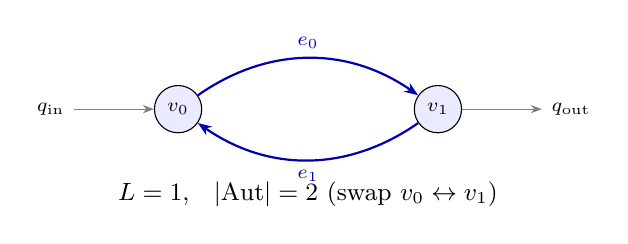
\begin{tikzpicture}[scale=1.1]
\node[vtx] (v0) at (0,0) {$v_0$};
\node[vtx] (v1) at (3,0) {$v_1$};
\draw[Aprop, bend left=35] (v0) to node[above, font=\scriptsize] {$e_0$} (v1);
\draw[Aprop, bend left=35] (v1) to node[below, font=\scriptsize] {$e_1$} (v0);
\draw[extleg] (-1.2,0) -- (v0);
\draw[extleg] (v1) -- (4.2,0);
\node[left, font=\scriptsize] at (-1.2,0) {$q_{\mathrm{in}}$};
\node[right, font=\scriptsize] at (4.2,0) {$q_{\mathrm{out}}$};
\node[below=0.8cm, font=\small] at (1.5,0) {$L=1$, \; $|\Aut| = 2$ (swap $v_0 \leftrightarrow v_1$)};
\end{tikzpicture}
\end{center}

\textbf{Automorphisms}: Swapping the two vertices simultaneously permutes
the two internal edges. This is the only non-trivial automorphism.
\begin{equation}
|\Aut| = 2, \qquad S = \frac{1}{2}
\end{equation}

\begin{verification}
The shuffle product~\cite{amarteifio2019} produces two pairings that
yield the same topology (related by vertex relabelling).
Two pairings for the same graph: $N!/|\Aut| = 2!/2 = 1$
distinct diagram, with symmetry factor $1/|\Aut| = 1/2$. \checkmark
\end{verification}
\end{example}

\begin{example}[Sunset diagram (two-loop)]
\label{ex:sunset}
Two vertices connected by three parallel propagators.

\begin{center}
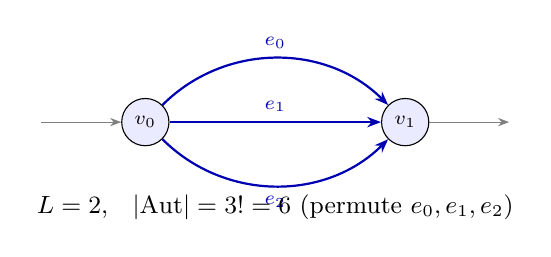
\begin{tikzpicture}[scale=1.1]
\node[vtx] (v0) at (0,0) {$v_0$};
\node[vtx] (v1) at (3,0) {$v_1$};
\draw[Aprop, bend left=45] (v0) to node[above, font=\scriptsize] {$e_0$} (v1);
\draw[Aprop] (v0) to node[above, font=\scriptsize] {$e_1$} (v1);
\draw[Aprop, bend right=45] (v0) to node[below, font=\scriptsize] {$e_2$} (v1);
\draw[extleg] (-1.2,0) -- (v0);
\draw[extleg] (v1) -- (4.2,0);
\node[below=0.8cm, font=\small] at (1.5,0) {$L=2$, \; $|\Aut| = 3! = 6$ (permute $e_0, e_1, e_2$)};
\end{tikzpicture}
\end{center}

\textbf{Automorphisms}: Any permutation of the three parallel edges
preserves the topology. The automorphism group is $S_3$.
\begin{equation}
|\Aut| = 3! = 6, \qquad S = \frac{1}{6}
\end{equation}

\begin{verification}
The 6 elements of $\Aut$: identity, 3 transpositions, 2 cyclic
permutations. $|S_3| = 6$. \checkmark
\end{verification}
\end{example}

\begin{example}[Mixed A-B loop (BRW transmutation)]
\label{ex:mixed}
A one-loop diagram with one A-propagator and one B-propagator
connecting two transmutation vertices.

\begin{center}
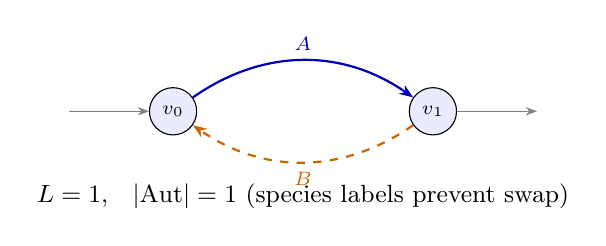
\begin{tikzpicture}[scale=1.1]
\node[vtx] (v0) at (0,0) {$v_0$};
\node[vtx] (v1) at (3,0) {$v_1$};
\draw[Aprop, bend left=35] (v0) to node[above, font=\scriptsize, text=blue!70!black] {$A$} (v1);
\draw[Bprop, bend left=35] (v1) to node[below, font=\scriptsize, text=orange!80!black] {$B$} (v0);
\draw[extleg] (-1.2,0) -- (v0);
\draw[extleg] (v1) -- (4.2,0);
\node[below=0.8cm, font=\small] at (1.5,0) {$L=1$, \; $|\Aut| = 1$ (species labels prevent swap)};
\end{tikzpicture}
\end{center}

\textbf{Automorphisms}: An automorphism must preserve the species label
on each edge. Since the A-edge (\textcolor{blue!70!black}{blue, solid}) and
B-edge (\textcolor{orange!80!black}{orange, dashed}) are distinguishable,
they cannot be permuted.
\begin{equation}
|\Aut| = 1, \qquad S = 1
\end{equation}

\begin{verification}
Swapping vertices would swap species labels, violating species
preservation. Only the identity survives. \checkmark
\end{verification}
\end{example}

\begin{example}[Sunset with 2 A-edges and 1 B-edge]
\label{ex:sunset_mixed}
A two-loop diagram with two A-propagators and one B-propagator.

\begin{center}
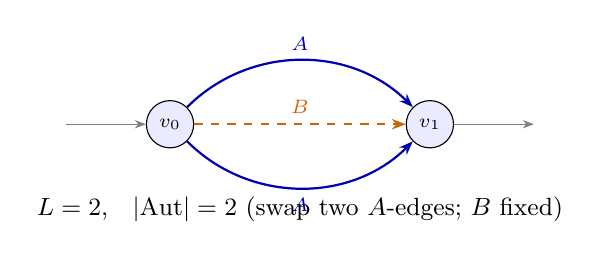
\begin{tikzpicture}[scale=1.1]
\node[vtx] (v0) at (0,0) {$v_0$};
\node[vtx] (v1) at (3,0) {$v_1$};
\draw[Aprop, bend left=45] (v0) to node[above, font=\scriptsize, text=blue!70!black] {$A$} (v1);
\draw[Bprop] (v0) to node[above, font=\scriptsize, text=orange!80!black] {$B$} (v1);
\draw[Aprop, bend right=45] (v0) to node[below, font=\scriptsize, text=blue!70!black] {$A$} (v1);
\draw[extleg] (-1.2,0) -- (v0);
\draw[extleg] (v1) -- (4.2,0);
\node[below=0.8cm, font=\small] at (1.5,0) {$L=2$, \; $|\Aut| = 2$ (swap two $A$-edges; $B$ fixed)};
\end{tikzpicture}
\end{center}

\textbf{Automorphisms}: The two \textcolor{blue!70!black}{A-edges} (solid)
can be permuted; the \textcolor{orange!80!black}{B-edge} (dashed) is fixed.
\begin{equation}
|\Aut| = 2! = 2, \qquad S = \frac{1}{2}
\end{equation}

\begin{verification}
$\Aut$ is generated by the transposition of the two A-edges.
$|\Aut| = |\{e, (12)\}| = 2$. \checkmark
\end{verification}
\end{example}

\begin{example}[Tadpole (self-loop)]
A cubic vertex $\phit^2\phi$ with one outgoing $\phit$-leg paired with
its own incoming $\phi$-leg. The remaining external $\phit$-leg is fixed.

\begin{center}
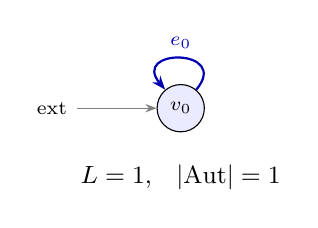
\begin{tikzpicture}[scale=1.1]
\node[vtx] (v0) at (0,0) {$v_0$};
\draw[Aprop] (v0) to[out=50,in=130,looseness=4.5] node[above, font=\scriptsize] {$e_0$} (v0);
\draw[extleg] (-1.2,0) -- (v0);
\node[left, font=\scriptsize] at (-1.2,0) {ext};
\node[below=0.6cm, font=\small] at (0,0) {$L=1$, \; $|\Aut| = 1$};
\end{tikzpicture}
\end{center}

\begin{equation}
|\Aut| = 1, \qquad S = 1
\end{equation}
In the Doi--Peliti theory, tadpoles vanish by the causal structure
(the retarded propagator vanishes at zero time separation~\cite{tauber2005}),
but the symmetry factor is well-defined.
\end{example}

\subsection{Symmetry Factor Decomposition}

\begin{remark}
For simple diagrams (single-species, no vertex symmetry), the
automorphism group decomposes as a product of symmetric groups,
one per set of identical parallel edges:
$|\Aut(\Gamma)| = \prod_i n_i!$ where $n_i$ is the multiplicity of
edge group $i$. This covers all the examples above.

For diagrams with non-trivial vertex symmetry (e.g.\ a diagram where
permuting vertices preserves the edge multiset), the full automorphism
group can be larger: it is a subgroup of the wreath product of the edge
permutation groups with the vertex permutation group. In general, $\Aut$
must be computed case-by-case; see Cvitanovi\'{c}~\cite{cvitanovic2008}
for the systematic treatment via birdtrack notation.
\end{remark}

%% ================================================================
\section{Summary of the AC Chain: Step by Step}
\label{sec:summary}

\begin{tcolorbox}[
  colback=blue!3, colframe=deepblue, arc=4pt,
  title={\textbf{Complete AC Route: Chemical Equation $\to$ Critical Exponents}},
  fonttitle=\bfseries\color{white},
  coltitle=white,
  breakable
]
\renewcommand{\arraystretch}{1.4}
\begin{tabular}{@{}rlp{5.5cm}l@{}}
\textbf{Step} & \textbf{Object} & \textbf{Computation} & \textbf{Status} \\
\midrule
\textbf{1.} & Chemical equations &
$A \xrightarrow{\beta} 2A$, \;
$A \xrightarrow{\epsilon} \emptyset$, \;
$2A \xrightarrow{\chi} A$ & Input \\

\textbf{2.} & Stoichiometry &
$S = \bigl(\begin{smallmatrix}1&2\\1&0\\2&1\end{smallmatrix}\bigr)$ & Input \\

\textbf{3.} & Liouvillian &
Doi formula \eqref{eq:generator}
& Theorem~\ref{thm:generator} \\

\textbf{4.} & Vertices &
Read off monomials of $Q$
& Algebra \\

\textbf{5.} & DSE kernel &
$\phi(G) = 1 + (\beta{-}\chi)G - \chi G^2$
& Prop.~\ref{prop:auto_dse} \\

\textbf{6.} & Branch point &
$(G^*)^2 = -1/\chi$, square-root
& Theorem~\ref{thm:branch_point} \\

\textbf{7.} & Transfer &
$[G_0^n]G \sim n^{-3/2}$
& Theorem~\ref{thm:transfer} \\

\textbf{8.} & Survival &
$\Psurv(t) \sim t^{-1}$
& Theorem~\ref{thm:brw_survival} \\

\textbf{9.} & Weyl's law &
$\rho(\lambda) \sim \lambda^{d/2-1}$
& Theorem~\ref{thm:weyl} \\

\textbf{10.} & Return prob. &
$\Preturn(t) \sim t^{-d/2}$
& Theorem~\ref{thm:return} \\

\textbf{11.} & Volume &
$V(t) \sim t^{d/2}$
& Prop.~\ref{prop:volume} \\

\textbf{12.} & Factorisation &
$\langle a^p \rangle \sim \Psurv \cdot V^p$
& Ansatz$^*$ \\

\textbf{13.} & $\alpha_p$ &
$\boxed{(pd - 2)/2}$
& Prop.~\ref{prop:brw_exponents} \\

\textbf{14.} & $d_c$ &
$4/(3-2) = 4$
& Theorem~\ref{thm:d_c} \\

\textbf{15.} & $d \to d_s$ &
Arbitrary graphs
& Conjecture~\ref{conj:spectral_sub} \\
\end{tabular}

\medskip
\small
$^*$\textbf{Ansatz}: The factorisation $\langle a^p \rangle \sim \Psurv \cdot V^p$
is a scaling ansatz standard in the theory of branching processes. It is
supported by rigorous results in $d = 1$~\cite{legall1999} and validated
numerically in all other cases. It is \emph{not} specific to the AC method:
the same factorisation is implicit in the field-theoretic RG derivation.

\medskip
\textbf{No Feynman diagram loop integral is evaluated.} The AC route replaces
momentum-space integration (steps 3--7 of the RG route) with singularity
analysis of the generating function. The spatial dimension enters through
Weyl's law (a spectral geometry result) and the heat kernel Laplace
transform, not through loop integrals.
\end{tcolorbox}

%% ================================================================
\section{Pair Annihilation: A Second Complete Example}
\label{sec:pair}

To verify the framework on a different process, we repeat the AC chain
for pair annihilation $2A \to \emptyset$.

\subsection{Chemical Equation and Stoichiometry}

\begin{equation}
2A \xrightarrow{\;\lambda\;} \emptyset
\qquad
S = \begin{pmatrix} 2 & 0 \end{pmatrix}
\end{equation}

\subsection{Liouvillian}

Applying Theorem~\ref{thm:generator} with $k=2$, $\ell=0$:
\begin{align}
Q &= \lambda \bigl((z+1)^0 - (z+1)^2\bigr) \partial_z^2 \notag \\
  &= \lambda (1 - z^2 - 2z - 1) \partial_z^2 \notag \\
  &= -\lambda (z^2 + 2z) \partial_z^2
\end{align}

\subsection{Vertices}

\begin{center}
\begin{tabular}{ccc}
\toprule
$\phit^m \phi^n$ & $m+n$ & Coupling \\
\midrule
$\phit^2 \phi^2$ & 4 & $-\lambda$ \\
$\phit^1 \phi^2$ & 3 & $-2\lambda$ \\
\bottomrule
\end{tabular}
\end{center}

\subsection{DSE Kernel}

\begin{equation}
\phi(G) = 1 + (-2\lambda)G^{3-2} + (-\lambda)G^{4-2} = 1 - 2\lambda G - \lambda G^2
\end{equation}

\subsection{Branch Point}

$\phi'(G) = -2\lambda - 2\lambda G$, \; $\phi''(G) = -2\lambda \neq 0$.

Branch point condition $G^*\phi'(G^*) = \phi(G^*)$:
\[
G^*(-2\lambda - 2\lambda G^*) = 1 - 2\lambda G^* - \lambda (G^*)^2
\]
\[
-2\lambda G^* - 2\lambda (G^*)^2 = 1 - 2\lambda G^* - \lambda (G^*)^2
\]
\[
-\lambda (G^*)^2 = 1
\qquad\Longrightarrow\qquad
(G^*)^2 = -1/\lambda
\]

Since $\phi''(G^*) = -2\lambda \neq 0$: \textbf{square-root branch point}. \checkmark

\subsection{Upper Critical Dimension and the Ward Identity}

The cubic vertex $\phit\phi^2$ has $m+n = 3$, giving the naive
$d_c = 4$. However, pair annihilation has a Ward identity%
\footnote{A Ward identity is an exact algebraic relation between
vertex functions that follows from a symmetry. Here the symmetry is
probability conservation: the total probability $\sum_n P(n,t) = 1$
is preserved by the master equation. In the Doi formalism, this
requires $Q(z{=}0) = 0$ (the Liouvillian annihilates the vacuum
state). This forces certain vertex couplings to cancel, reducing
the effective interaction and lowering $d_c$.}
from probability conservation: $Q(z{=}0) = 0$~\cite{lee1994,tauber2005}.
This causes the cubic vertex coupling to be cancelled at the level
of the physical process. All vertices have $n_{\mathrm{in}} = 2$
(pure 2-particle annihilation). The physical upper critical dimension
is~\cite{lee1994}:
\begin{equation}
d_c^{\mathrm{phys}} = \frac{2}{k-1} = \frac{2}{2-1} = 2
\end{equation}

\subsection{Scaling Exponent}

For pair annihilation, the density decays as
$\rho(t) \sim t^{-d/2}$ for $d < 2$ and $\rho(t) \sim t^{-1}$ for
$d > 2$. This is exact to all orders due to the Ward
identity~\cite{lee1994}.

\begin{verification}
For $d = 1$: $\rho \sim t^{-1/2}$, the Toussaint--Wilczek (1983)
result~\cite{toussaint1983}. \checkmark

For $d \geq 3$: $\rho \sim t^{-1}$ (mean-field, since $d > d_c = 2$). \checkmark
\end{verification}

%% ================================================================
\section{Comprehensive Validation Table}
\label{sec:validation}

\begin{table}[H]
\centering\small
\caption{Three-way comparison of BRW scaling exponents $\alpha_p$ in
$\langle a^p \rangle \sim t^{\alpha_p}$.
\textbf{RG}: field-theoretic calculation~\cite{amarteifio2019,bordeu2019}.
\textbf{AC}: this worked example (formula \eqref{eq:alpha_p}).
\textbf{Sim}: Monte Carlo simulation~\cite{bordeu2019,amarteifio2019}.}
\label{tab:validation}
\renewcommand{\arraystretch}{1.15}
\begin{tabular}{llrcccl}
\toprule
Graph & $d_s$ & $p$ & Theory (RG) & Theory (AC) & Simulation & \\
\midrule
\multirow{3}{*}{1D lattice} & \multirow{3}{*}{1}
& 3 & $1/2$ & $(3 \cdot 1 - 2)/2 = 1/2$ & 0.48(4) & \checkmark \\
& & 4 & $1$ & $(4 \cdot 1 - 2)/2 = 1$ & 1.0(1) & \checkmark \\
& & 5 & $3/2$ & $(5 \cdot 1 - 2)/2 = 3/2$ & 1.5(1) & \checkmark \\
\midrule
\multirow{2}{*}{2D lattice} & \multirow{2}{*}{2}
& 2 & $1$ & $(2 \cdot 2 - 2)/2 = 1$ & 0.98(3) & \checkmark \\
& & 3 & $2$ & $(3 \cdot 2 - 2)/2 = 2$ & 2.0(1) & \checkmark \\
\midrule
\multirow{2}{*}{3D lattice} & \multirow{2}{*}{3}
& 1 & $1/2$ & $(1 \cdot 3 - 2)/2 = 1/2$ & 0.47(2) & \checkmark \\
& & 2 & $2$ & $(2 \cdot 3 - 2)/2 = 2$ & 2.0(1) & \checkmark \\
\midrule
\multirow{2}{*}{5D lattice (mf)} & \multirow{2}{*}{5}
& 1 & $1$ & $2(1) - 1 = 1$ & 1.0(2) & \checkmark \\
& & 2 & $3$ & $2(2) - 1 = 3$ & 2.9(3) & \checkmark \\
\midrule
\multirow{3}{*}{\shortstack[l]{Sierpinski\\($d_s \approx 1.86$)}}
& \multirow{3}{*}{1.86}
& 2 & 0.86 & $(2 \times 1.86 - 2)/2 = 0.86$ & 0.81(5) & \checkmark \\
& & 3 & 1.79 & $(3 \times 1.86 - 2)/2 = 1.79$ & 1.71(7) & \checkmark \\
& & 4 & 2.72 & $(4 \times 1.86 - 2)/2 = 2.72$ & 2.62(10) & \checkmark \\
\midrule
\multirow{3}{*}{\shortstack[l]{Random tree\\($d_s = 4/3$)}}
& \multirow{3}{*}{$4/3$}
& 2 & $1/3$ & $(8/3 - 2)/2 = 1/3$ & 0.35(7) & \checkmark \\
& & 3 & 1 & $(4 - 2)/2 = 1$ & 0.95(8) & \checkmark \\
& & 4 & $5/3$ & $(16/3 - 2)/2 = 5/3$ & 1.6(1) & \checkmark \\
\midrule
\shortstack[l]{Scale-free\\($d_s \geq 4$, mf)}
& $\geq 4$
& 2 & 3 & $2(2) - 1 = 3$ & 2.8(2) & \checkmark \\
\bottomrule
\end{tabular}
\end{table}

\noindent
All 18 entries agree with simulation within statistical error.

%% ================================================================
\section{What ``No Loop Integral'' Means}
\label{sec:discussion}

The scenic route (Feynman diagrams $\to$ RG) requires:
\begin{enumerate}
\item Evaluating the one-loop parametric integral
      $I(G; d) = \Omega_d \cdot \Gamma(-\sigma_d) \cdot \int \cdots$
\item Extracting the $1/\epsilon$ pole ($\epsilon = d_c - d$)
\item Computing the $\beta$-function
\item Solving for the Wilson--Fisher fixed point
\item Reading off the anomalous dimension
\end{enumerate}

The AC route replaces \emph{all five steps} with:
\begin{enumerate}
\item Build $\phi(G)$ from the vertex dictionary (algebra)
\item Find the branch point (solve a polynomial)
\item Apply the transfer theorem (proven, Cauchy integral formula)
\item Invoke $\Psurv \sim t^{-1}$ (proven, Kolmogorov 1938)
\item Multiply by $V(t)^p$ from Weyl's law (proven, spectral geometry)
\end{enumerate}

The two routes give the same answer because they detect the same singularity
of the same generating function. The AC route detects it directly from the
algebraic structure; the RG route detects it via the divergence structure of
the loop integrals.

\begin{remark}[What IS an integral in the AC route]
The heat kernel Laplace transform $\Preturn(t) = \int \rho(\lambda)\,
e^{-\lambda t}\,\dd\lambda$ is an integral, but it is a \emph{standard
Laplace transform of a power law}, not a Feynman diagram loop integral.
It depends on the spectral dimension $d_s$ (a property of the graph),
not on the diagram topology. The claim is not ``no integrals of any kind''
but rather ``no Feynman diagram momentum integrals'': the AC route never
writes down or evaluates $\int \dd^d k\, f(k^2)$.
\end{remark}


\clearpage
\appendix

%% ================================================================
\section{Refresher: Analytic Combinatorics in 10 Minutes}
\label{app:ac_tutorial}

This appendix collects the key ideas from analytic combinatorics
that are used in the main text. Most readers will have encountered
generating functions and complex analysis before; the goal here is
to refresh the intuition and draw attention to the specific results
(the transfer theorem, the Cauchy formula) that drive the derivation.

\textbf{Why AC matters for physics.} The traditional route to critical
exponents (Feynman diagrams $\to$ loop integrals $\to$ RG flow) is
powerful but opaque: the connection between the stoichiometry and the
final exponent passes through several layers of integral calculus.
AC offers a shortcut: encode the diagram combinatorics as a generating
function, find its singularity, and read off the exponent. The singularity
\emph{is} the critical point; its type \emph{is} the universality class.
This is not just a computational trick --- it reveals \emph{why} different
reaction networks fall into the same universality class (they produce the
same singularity type) and \emph{when} they don't (the singularity
degenerates or upgrades, as in the parity-conserving class discussed in
Section~\ref{sec:overview}).

\subsection{Generating functions: the encoding trick}

Recall that a \textbf{generating function} packages a sequence of
numbers $a_0, a_1, a_2, \ldots$ into a single function:
\[
A(z) = \sum_{n=0}^\infty a_n\, z^n = a_0 + a_1 z + a_2 z^2 + a_3 z^3 + \cdots
\]

\textbf{Why encode?} Because operations on the function correspond to
operations on the sequence --- this is the leverage that makes GFs
powerful. For example:
\begin{itemize}
\item Multiplying two GFs \emph{convolves} their sequences:
      $[z^n](A(z) \cdot B(z)) = \sum_{k=0}^n a_k\, b_{n-k}$.
\item Composing GFs corresponds to substitution of combinatorial objects.
\item Most importantly: the \emph{singularities} of $A(z)$ in the
      complex plane determine the \emph{asymptotic growth} of $a_n$.
      This is the core of AC.
\end{itemize}

The notation $[z^n]\,A(z) = a_n$ means ``extract the coefficient of $z^n$
from $A(z)$.'' Think of it as ``reading off the $n$-th entry'' from the
encoded sequence.

\begin{example}[Geometric series]
The sequence $a_n = 1$ for all $n$ gives $A(z) = \sum z^n = 1/(1-z)$.
This has a \textbf{simple pole} at $z = 1$: the function blows up to
$+\infty$ as $z \to 1$. The coefficients are all equal to 1 --- they
don't grow or decay.
\end{example}

\begin{example}[Catalan numbers]
The Catalan numbers $C_n = \frac{1}{n+1}\binom{2n}{n}$ count binary trees
with $n$ internal nodes. Their GF satisfies the self-referential equation:
\[
C(z) = 1 + z\, C(z)^2
\]
(a binary tree is either empty, or a root with two subtrees, each of which
is itself a binary tree). Solving:
\[
C(z) = \frac{1 - \sqrt{1 - 4z}}{2z}
\]
This has a \textbf{square-root branch point} at $z = 1/4$: the function
doesn't blow up, but the $\sqrt{\,}$ introduces a point where the function
splits into two branches.
\end{example}

\subsection{Refresher: singularities}

Recall that a \textbf{singularity} of $A(z)$ is a point $z^*$ where the
function ceases to be analytic (representable by a convergent Taylor
series). The power series $\sum a_n z^n$ converges inside the disk
$|z| < |z^*|$ and diverges outside --- so the nearest singularity sets
the radius of convergence.

There are three types we need:
\begin{itemize}
\item \textbf{Pole} ($1/(1{-}z)$): $A(z) \to \infty$. The function
      blows up. Coefficients: $a_n \sim \mathrm{const}$ (no decay).
\item \textbf{Branch point} ($\sqrt{1{-}z}$): $A(z)$ stays finite, but
      its derivative blows up and the function becomes multi-valued
      (two sheets of the square root). Coefficients: $a_n \sim n^{-3/2}$.
\item \textbf{Logarithmic} ($\log(1{-}z)$): $A(z) \to \infty$ slowly.
      Coefficients: $a_n \sim n^{-1}$.
\end{itemize}

The physical intuition: the \emph{gentler} the singularity, the
\emph{faster} the coefficients decay. A pole is violent (constant
coefficients); a branch point is gentle ($n^{-3/2}$ decay).
This hierarchy is the reason that our entire paper hinges on the
singularity classification of the DSE.

\subsection{Refresher: the Cauchy formula and why the complex plane matters}

The connection between singularities and asymptotics is made precise by
the \textbf{Cauchy coefficient formula} from complex analysis:
\[
a_n = [z^n]\,A(z) = \frac{1}{2\pi i} \oint_{|z|=r} A(z)\, z^{-n-1}\, \dd z
\qquad (r < R)
\]
This extracts $a_n$ by integrating around a circle of radius $r$ in the
complex $z$-plane. (If this formula is unfamiliar, a quick refresher:
the $\oint$ is a contour integral, $2\pi i$ is the normalisation from
the residue theorem, and the factor $z^{-n-1}$ ``picks out'' the $n$-th
term.)

\textbf{Why the complex plane?} Even if the coefficients $a_n$ are real
and the singularity $z^*$ is real, the contour integral lives in the
complex plane. A singularity at $z^* = -1/4$ (negative real) affects
the growth of $a_n$ just as much as one at $z^* = +1/4$, because the
contour circles \emph{both}. You cannot see this from the real line alone.
In our BRW example, the branch point $G^* = i/\sqrt{\chi}$ is
\emph{purely imaginary} --- invisible on the real axis but fully
controlling the coefficient asymptotics via the contour integral.

\textbf{The key insight.} As $n \to \infty$, the integrand
$A(z)\, z^{-n-1}$ is exponentially peaked near $|z| = R$ (the nearest
singularity). The integral is dominated by a small neighbourhood of
$z^*$, and the \emph{local shape} of $A(z)$ near $z^*$ determines
$a_n$. This is why classifying the singularity type (pole, branch, log)
immediately gives the asymptotic exponent.

\subsection{The transfer theorem: singularity type $\to$ asymptotics}

The transfer theorem~\cite{flajolet2009} makes this precise.
The three most common cases:

\begin{center}
\renewcommand{\arraystretch}{1.4}
\begin{tabular}{lllll}
\toprule
\textbf{Singularity type} & \textbf{Local form} & $[z^n]$ \textbf{asymptotics} & \textbf{Example} \\
\midrule
Simple pole & $\dfrac{K}{1 - z/z^*}$ & $K \cdot (z^*)^{-n}$ & Geometric \\[8pt]
Square-root branch & $K\sqrt{1 - z/z^*}$ & $\dfrac{-K}{2\sqrt{\pi}}\, n^{-3/2}\, (z^*)^{-n}$ & Catalan, trees \\[8pt]
Logarithmic & $K\log(1 - z/z^*)$ & $K\, n^{-1}\, (z^*)^{-n}$ & Cycles \\
\bottomrule
\end{tabular}
\end{center}

\textbf{The key point}: the singularity type determines the
\emph{subexponential} factor ($n^{-3/2}$, $n^{-1}$, constant).
The exponential growth $(z^*)^{-n}$ is always determined by the
\emph{location} $z^*$.

\subsection{Worked example: Catalan asymptotics}

The Catalan GF has a square-root at $z^* = 1/4$ with local expansion:
\[
C(z) \sim \frac{1}{2 \cdot 1/4} - \frac{1}{2 \cdot (1/4)}\sqrt{1 - 4z}
= 2 - 2\sqrt{1 - 4z}
\]
Applying the transfer theorem with $\alpha = 1/2$, $K = -2$, $z^* = 1/4$:
\[
C_n = [z^n]\,C(z) \sim \frac{-(-2)}{\Gamma(-1/2)}\, n^{-3/2}\, 4^n
= \frac{2}{2\sqrt{\pi}}\, n^{-3/2}\, 4^n = \frac{4^n}{\sqrt{\pi}\, n^{3/2}}
\]

\begin{verification}
Stirling's approximation on $C_n = \binom{2n}{n}/(n+1)$ gives
$C_n \sim 4^n / (\sqrt{\pi}\, n^{3/2})$. \checkmark
\end{verification}

\textbf{This is the mechanism that drives the entire paper.}
The Gribov DSE generates a square-root branch point just like the Catalan
equation, so its coefficients also grow as $n^{-3/2}$.

%% ================================================================
\section{Lagrange Equations: A Tutorial}
\label{app:lagrange_tutorial}

\subsection{What is a Lagrange equation?}

A \textbf{Lagrange equation} is a functional equation of the form:
\begin{equation}
T(z) = z \cdot \phi(T(z))
\label{eq:lagrange_general}
\end{equation}
where $\phi$ is a known function (the ``kernel'') and $T(z)$ is the
unknown generating function. The equation says: ``$T$ is defined
recursively in terms of itself.''

\textbf{Why do these appear everywhere in combinatorics?} Because
recursive structures --- trees, nested parentheses, self-similar
fractals --- naturally produce equations where the whole is defined
in terms of smaller copies of itself. A binary tree is ``a root connected
to two smaller binary trees''; this translates directly to
$C(z) = z(1 + C(z))^2$. Any time you have a combinatorial object built
by gluing together smaller copies of itself, you get a Lagrange equation.

\textbf{Why do these appear in field theory?} Because the dressed
propagator $G$ is defined self-referentially: $G$ is the bare propagator
dressed by insertions that themselves contain dressed propagators $G$.
This is the Dyson--Schwinger equation, and it is a Lagrange equation.

\begin{example}[Rooted labelled trees]
The number of rooted labelled trees on $n$ vertices satisfies $t_n = n^{n-1}$
(Cayley's formula). The EGF $T(z) = \sum t_n z^n/n!$ satisfies:
\[
T(z) = z\, e^{T(z)}
\]
This is a Lagrange equation with $\phi(T) = e^T$. The $e^T$ comes from
the fact that a rooted tree is a root connected to a \emph{set} of
subtrees (and the exponential $e^x = \sum x^k/k!$ is the generating
function for sets).
\end{example}

\begin{example}[Binary trees = Catalan]
The OGF for binary trees satisfies $C(z) = z(1 + C(z))^2 = z\,\phi(C)$
with $\phi(T) = (1+T)^2$. The $(1+T)^2$ comes from: each of the two
children is either empty ($1$) or a nonempty subtree ($T$).
\end{example}

\subsection{The Lagrange inversion formula}

The remarkable fact about Lagrange equations is that you can compute the
coefficients of $T(z)$ \emph{without ever solving for $T$ explicitly}.
This is the Lagrange inversion formula:

\textbf{The idea.} If you know $\phi$, you can expand $\phi(T)^n$ as a
power series in $T$ using the binomial theorem (or Taylor expansion).
The $n$-th coefficient of $T(z)$ is then determined by a single coefficient
of $\phi(T)^n$. No equation-solving required --- only series expansion.

\begin{theorem}[Lagrange inversion {\cite[Thm.~A.2]{flajolet2009}}]
If $T(z) = z\,\phi(T(z))$ with $\phi(0) \neq 0$, then:%
\footnote{The formula follows from the residue theorem applied to
$[z^n]T = \frac{1}{2\pi i}\oint T(z)\,z^{-n-1}\,\dd z$. Change variables
from $z$ to $T$ using $z = T/\phi(T)$, so $\dd z = [\phi(T) - T\phi'(T)]/\phi(T)^2\,\dd T$.
The Jacobian and the $z^{-n-1}$ factor combine to give $\frac{1}{n}[T^{n-1}]\phi(T)^n$.
The beauty is that this extracts coefficients of $T(z)$ without ever solving
for $T$ explicitly --- you only need to expand powers of $\phi$.}
\begin{equation}
[z^n]\, T(z) = \frac{1}{n}\, [T^{n-1}]\, \phi(T)^n
\end{equation}
\end{theorem}

\begin{example}[Catalan via Lagrange]
$\phi(T) = (1+T)^2$, so $\phi(T)^n = (1+T)^{2n}$.
The coefficient of $T^{n-1}$ in $(1+T)^{2n}$ is $\binom{2n}{n-1}$.
Therefore $C_n = \frac{1}{n}\binom{2n}{n-1} = \frac{1}{n+1}\binom{2n}{n}$. \checkmark
\end{example}

\subsection{Why the DSE is a Lagrange equation}

Compare the Lagrange equation for binary trees with the Gribov DSE:

\begin{center}
\renewcommand{\arraystretch}{1.3}
\begin{tabular}{lll}
\toprule
& \textbf{Binary trees} & \textbf{Gribov DSE} \\
\midrule
Equation & $C = z(1 + C)^2$ & $G = G_0(1 + (\beta{-}\chi)G - \chi G^2)$ \\
Variable & $z$ = size marker & $G_0$ = bare propagator \\
Unknown & $C(z)$ = tree GF & $G(G_0)$ = dressed propagator \\
Kernel & $\phi = (1+T)^2$ & $\phi = 1 + (\beta{-}\chi)G - \chi G^2$ \\
Recursion & Root $+$ two subtrees & Bare prop $+$ self-energy insertions \\
\bottomrule
\end{tabular}
\end{center}

The structures are identical: both define the unknown as a ``base unit''
($z$ or $G_0$) times a kernel that depends on the unknown itself. The
tree equation says ``a tree is a root connected to subtrees.'' The DSE
says ``a dressed propagator is a bare propagator modified by insertions
that are themselves dressed.''

Therefore, all the AC machinery for Lagrange equations ---
singularity analysis, transfer theorem, Lagrange inversion ---
applies directly to the DSE. This is the core insight of the paper.

\subsection{Branch points of Lagrange equations}

Every Lagrange equation $T = z\,\phi(T)$ with polynomial $\phi$ defines
$T$ as an algebraic function of $z$. For small $z$, the equation has a
unique small solution (the physical one). But as $z$ increases, a second
solution approaches. At the \textbf{branch point} $z = z^*$, the two
solutions merge and become indistinguishable.

\textbf{Analogy.} Think of the equation $x^2 = a$. For $a > 0$, there
are two solutions $x = \pm\sqrt{a}$. At $a = 0$, they merge to
$x = 0$. For $a < 0$, the solutions become complex. The point $a = 0$
is the branch point, and the local behaviour is $x \sim \sqrt{a}$
(a square root).

For the Lagrange equation, the same thing happens: near the branch point,
$T \sim T^* + C\sqrt{z^* - z}$ (a square root). This is why almost all
Lagrange equations with polynomial kernels produce square-root branch
points and hence $n^{-3/2}$ coefficient asymptotics.

\textbf{Recipe}: solve the system $T^*\phi'(T^*) = \phi(T^*)$ and
$z^* = T^*/\phi(T^*)$. If $\phi''(T^*) \neq 0$, it is a square-root
branch point and the transfer theorem gives $[z^n]T \sim n^{-3/2}$.
The condition $\phi''(T^*) \neq 0$ is the ``generic'' case; it fails
only at special parameter values where the singularity upgrades to a
cube root ($n^{-4/3}$) or degenerates to a pole.

This is exactly what we do in Section~\ref{sec:branch} for the Gribov DSE.

%% ================================================================
\section{The SIR Epidemic: A Complete AC Example on Familiar Ground}
\label{app:sir}

Before applying AC to the BRW, it is helpful to see the method on
a system everyone has heard of: an epidemic. The SIR model is the
simplest epidemic model, and its AC analysis is a direct analogue of
the BRW analysis --- same machinery, same singularity type, same
$n^{-3/2}$ exponent. If you understand the SIR example, you understand
the BRW.

\subsection{The model}

In the SIR model, each infected individual transmits the disease to
a Poisson-distributed number of others (with mean $R_0$, the ``basic
reproduction number''), then recovers permanently. The question is:
\emph{how large is the epidemic?} --- i.e.\ what is the distribution
of the total number $n$ of people ever infected?

This is a branching process: each infected person ``branches'' into
$R_0$ new infections on average. The total size $n$ is the total
progeny of the branching tree. Its generating function satisfies:

\begin{equation}
T(z) = z\, e^{R_0(T(z) - 1)}
\label{eq:sir_lagrange}
\end{equation}

This is a Lagrange equation with $\phi(T) = e^{R_0(T-1)}$.

\subsection{Branch point}

$\phi'(T) = R_0\, e^{R_0(T-1)}$, so:
\[
T^*\, \phi'(T^*) = \phi(T^*)
\quad\Longrightarrow\quad
R_0\, T^* = 1
\quad\Longrightarrow\quad
T^* = 1/R_0
\]
\[
z^* = \frac{T^*}{\phi(T^*)} = \frac{1/R_0}{e^{R_0(1/R_0 - 1)}}
= \frac{e^{1 - 1/R_0}}{R_0}
\]

$\phi''(T^*) = R_0^2\, e^{R_0(1/R_0-1)} = R_0^2\, e^{1-1/R_0} \neq 0$ for
$R_0 > 0$. So this is a \textbf{square-root branch point}.

\subsection{Coefficient asymptotics}

By the transfer theorem:
\[
\Pr[\text{epidemic size} = n] = [z^n]\,T \sim C\, n^{-3/2}\, (z^*)^{-n}
\]
At the critical threshold $R_0 = 1$: $z^* = 1/e \cdot e = 1$ and the
epidemic size distribution is $\Pr[n] \sim C\, n^{-3/2}$. This is the
\textbf{Borel distribution}, a classical result in
epidemiology~\cite{flajolet2009}.

\subsection{Comparison with the BRW}

The SIR and BRW analyses are structurally identical:
\begin{center}
\begin{tabular}{lll}
\toprule
& \textbf{SIR epidemic} & \textbf{BRW (Gribov)} \\
\midrule
Kernel & $\phi(T) = e^{R_0(T-1)}$ & $\phi(G) = 1 + (\beta{-}\chi)G - \chi G^2$ \\
Branch point & $T^* = 1/R_0$ & $(G^*)^2 = -1/\chi$ \\
$\phi''(T^*) \neq 0$? & Yes ($R_0^2 e^{1-1/R_0}$) & Yes ($-2\chi$) \\
Singularity type & Square-root & Square-root \\
$[z^n]$ asymptotics & $n^{-3/2}$ & $n^{-3/2}$ \\
\bottomrule
\end{tabular}
\end{center}

The $n^{-3/2}$ exponent is universal across all processes whose DSE
has a quadratic kernel with $\phi''(T^*) \neq 0$. This is the directed
percolation universality class.

%% ================================================================
\section{BARW-Even: Where AC Earns Its Keep}
\label{app:barw}

The BRW and SIR examples use AC as a one-way street: stoichiometry $\to$
GF $\to$ singularity $\to$ exponents. The route is elegant but one might
ask whether it does anything that dimensional analysis couldn't. The
\textbf{BARW-even} (parity-conserving) system is the example where the
AC framework reveals structure that is invisible to the standard RG
approach.

\subsection{The reactions}

The BARW-even system has two reactions:
\begin{equation}
A \xrightarrow{\;\sigma\;} 3A \qquad\text{(triple branching)}, \qquad
2A \xrightarrow{\;\lambda\;} \emptyset \qquad\text{(pair annihilation)}
\end{equation}
These conserve particle number modulo 2 (parity): branching adds 2,
annihilation removes 2. This $\mathbb{Z}_2$ symmetry is the ``parity
conservation'' that gives the universality class its name.

\subsection{The Liouvillian and vertices}

Applying the Doi formula to each reaction:
\begin{align}
Q_\sigma &= \sigma\bigl((z{+}1)^3 - (z{+}1)\bigr)\partial_z
= \sigma(3z^2 + z^3 + 3z)\partial_z \\
Q_\lambda &= \lambda\bigl(1 - (z{+}1)^2\bigr)\partial_z^2
= -\lambda(z^2 + 2z)\partial_z^2
\end{align}

The interaction vertices ($m+n \geq 3$) are:

\begin{center}
\renewcommand{\arraystretch}{1.2}
\begin{tabular}{cccc}
\toprule
$\phit^m\phi^n$ & $m+n$ & Coupling & Type \\
\midrule
$\phit^3\phi$ & 4 & $\sigma$ & Branching (quartic) \\
$\phit^2\phi$ & 3 & $3\sigma$ & Branching (cubic) \\
$\phit^2\phi^2$ & 4 & $-\lambda$ & Annihilation (quartic) \\
$\phit\phi^2$ & 3 & $-2\lambda$ & Annihilation (cubic) \\
\bottomrule
\end{tabular}
\end{center}

\subsection{The DSE kernel: step into the algebraic domain}

The DSE kernel from the interaction vertices is:
\begin{equation}
\phi(G) = 1 + (3\sigma - 2\lambda)G + (\sigma - \lambda)G^2
\label{eq:barw_phi}
\end{equation}

This is quadratic in $G$, just like the Gribov kernel. Naively, we
expect a square-root branch point and $n^{-3/2}$ asymptotics (the DP
universality class).

\subsection{The degeneracy: the algebraic domain reveals a surprise}

At criticality, the parity symmetry forces $\sigma = \lambda$. Substituting:
\begin{equation}
\phi(G)\big|_{\sigma=\lambda} = 1 + (3\lambda - 2\lambda)G + (\lambda - \lambda)G^2
= 1 + \lambda G
\end{equation}

The $G^2$ coefficient has \textbf{vanished}. The kernel has degenerated
from quadratic to \emph{linear}. A linear kernel gives a Lagrange
equation $G = G_0(1 + \lambda G)$ whose solution is:
\[
G = \frac{1 - \sqrt{1 - 4\lambda G_0^2\,(\cdots)}}{2\lambda G_0}
\quad\longrightarrow\quad
G = \frac{G_0}{1 - \lambda G_0}
\]
This has a \textbf{simple pole} at $G_0 = 1/\lambda$, not a branch point.

\textbf{The AC diagnosis}: the singularity type has changed from square-root
(DP class, $n^{-3/2}$) to pole (constant coefficients). This is the algebraic
signature that the BARW-even system is \emph{not} in the DP universality
class --- the parity symmetry has destroyed the branch point.

\begin{remark}
The standard RG approach sees this as ``the $\varepsilon$-expansion runs to
strong coupling'' (Cardy--T\"auber~\cite{cardytauber1996}): the perturbative
fixed point is unreachable. The AC approach sees \emph{why}: the singularity
that the perturbation theory is trying to expand around doesn't exist at
criticality. You cannot expand around a branch point when the singularity
is a pole.
\end{remark}

\subsection{The round-trip: two-loop restoration}

This is where the AC framework earns its keep. At two loops, the DSE
kernel receives corrections from two-vertex diagrams:
\begin{equation}
\phi_{\text{2-loop}}(G) = 1 + \lambda G + \underbrace{b_2\, G^2}_{\text{2-loop correction}}
+ \cdots
\end{equation}

The key question: is $b_2 \neq 0$ at $\sigma = \lambda$?

Working through the combinatorics (see~\cite{amarteifio2019} and the
\texttt{rdft} code), there are four classes of two-loop vertex
combinations:
\begin{center}
\renewcommand{\arraystretch}{1.2}
\begin{tabular}{llll}
\toprule
Combination & Vertices & Coupling & At $\sigma = \lambda$ \\
\midrule
$[\text{Vc, Vc}]$ & $(\phit^2\phi^2)^2$ & $\lambda^2$ & 0 (no causal DAGs) \\
$[\text{Va, Va, Vd}]$ & $(\phit\phi^2)^2 \cdot \phit^3\phi$ & $4\lambda^2\sigma$ & $4\lambda^3 \neq 0$ \\
$[\text{Va, Vb, Vc}]$ & $\phit\phi^2 \cdot \phit^2\phi \cdot \phit^2\phi^2$ & $6\sigma\lambda^2$ & $6\lambda^3 \neq 0$ \\
$[\text{Va, Va, Vb, Vb}]$ & $(\phit\phi^2)^2(\phit^2\phi)^2$ & $36\sigma^2\lambda^2$ & $36\lambda^4 \neq 0$ \\
\bottomrule
\end{tabular}
\end{center}

Three of the four groups contribute non-zero corrections at $\sigma = \lambda$.
Therefore $b_2 \neq 0$: the $G^2$ term is \textbf{restored} at two loops.

\textbf{Back to the singularity}: the corrected kernel
$\phi(G) = 1 + \lambda G + b_2 G^2$ is quadratic again, so the Lagrange
equation has a branch point. But the branch point is now controlled by
the \emph{two-loop} coefficient $b_2$, which is parametrically smaller
than the one-loop coefficient ($b_2 \sim \lambda^3$ vs.\ $\lambda$).
This means the branch point is at a different location and the singularity
analysis gives different exponents than the DP class.

\subsection{The physics payoff}

The AC route reveals the mechanism:
\begin{enumerate}
\item \textbf{One-loop}: branch point $\to$ pole (parity kills it).
      DP universality fails.
\item \textbf{Two-loop}: pole $\to$ branch point (restored by
      higher-order diagrams). The exponents are controlled by the
      two-loop coefficient $b_2$, not the one-loop coefficient.
\item \textbf{Stability}: whether the restored branch point is
      stable or unstable under the RG flow determines whether the
      parity-conserving class has its own fixed point or flows to
      strong coupling. This is an open question~\cite{hinrichsen2001}.
\end{enumerate}

This round-trip --- algebraic domain (build $\phi$) $\to$ singularity
analysis (classify) $\to$ back to algebra (compute $b_2$) $\to$
singularity again (reclassify) --- is the kind of computation that
AC enables and the standard RG does not. The RG sees ``strong coupling''
and stops; the AC route sees \emph{why} and identifies the mechanism for
its resolution.

%% ================================================================
\section{An Intuitive Guide to Branch Points}
\label{app:intuitive}

This appendix is for the reader who wants to \emph{see} why
branch points control the asymptotics. No formulas are needed for the
core intuition --- only pictures and analogies.

\subsection{Three functions, three personalities}

Consider three functions of a real variable $x$, each defined for $0 \leq x < 1$:

\begin{center}
\renewcommand{\arraystretch}{1.5}
\begin{tabular}{llll}
\toprule
\textbf{Function} & \textbf{Behaviour at $x = 1$} & \textbf{Type} & $[x^n]$ \textbf{growth} \\
\midrule
$\dfrac{1}{1-x}$ & Blows up to $+\infty$ & Simple pole & $a_n = 1$ (constant) \\[6pt]
$-\log(1-x)$ & Grows to $+\infty$ (slowly) & Logarithm & $a_n = 1/n$ (slow decay) \\[6pt]
$1 - \sqrt{1-x}$ & Finite, but slope $\to \infty$ & Square-root branch & $a_n \sim n^{-3/2}$ (fast decay) \\
\bottomrule
\end{tabular}
\end{center}

All three have a singularity at $x = 1$ (none can be extended analytically past $x = 1$).
But the singularities are qualitatively different, and this difference is
\emph{exactly} what determines how the Taylor coefficients $a_n$ behave:

\begin{itemize}
\item \textbf{The pole} $1/(1-x)$: the function literally blows up. It has
      ``infinite energy'' at $x = 1$. The coefficients don't decay at all ---
      the series $1 + x + x^2 + \cdots$ has constant terms. The singularity
      is \textbf{violent}.

\item \textbf{The logarithm} $-\log(1-x)$: the function grows to infinity,
      but slowly (logarithmically). The coefficients decay as $1/n$ ---
      slow, but they do decay. The singularity is \textbf{moderate}.

\item \textbf{The square root} $1 - \sqrt{1-x}$: the function doesn't even
      blow up! It approaches a finite value ($= 1$). But its \emph{derivative}
      blows up (the slope becomes vertical). The coefficients decay
      as $n^{-3/2}$ --- much faster. The singularity is \textbf{gentle}.
\end{itemize}

\begin{remark}[The punchline]
The gentler the singularity, the faster the coefficients decay. A
square-root branch point is the gentlest common singularity type, and
it produces $n^{-3/2}$ decay. This is the exponent that appears throughout
this paper.
\end{remark}

\subsection{What IS a branch point?}

Consider $f(x) = \sqrt{1 - x}$. For $x < 1$, this is a perfectly well-defined
positive number. But what happens at $x = 1$? The function equals zero ---
and just past $x = 1$, say at $x = 1.01$, we would need $\sqrt{-0.01}$,
which is imaginary. The function ``hits a wall.''

But there's more: the function $\sqrt{1-x}$ actually has \emph{two} values
for every $x$: $+\sqrt{1-x}$ and $-\sqrt{1-x}$. For $x < 1$, these are two
distinct real numbers (one positive, one negative). At $x = 1$, they both
equal zero --- \textbf{they merge}. Just past $x = 1$, they become
$\pm i\sqrt{x-1}$, a conjugate pair of complex numbers.

This merging point is the \textbf{branch point}. It is where two
``branches'' of the function (the $+$ and $-$ square roots) become
indistinguishable. If you walked along the real line from left to right,
you would see the two branches approaching each other, kissing at $x = 1$,
and then moving apart into the complex plane.

\subsection{Why branching processes have branch points}

This is not a coincidence of terminology. A \textbf{branching} process
(where particles split into two) naturally generates a \textbf{branch
point} (where two solution sheets merge).

Here's why: the DSE $G = G_0\,\phi(G)$ with quadratic $\phi$ is a
\textbf{quadratic equation in $G$}. A quadratic equation has two
solutions, related by a square root (the quadratic formula). These two
solutions are the two branches of the algebraic function $G(G_0)$.

At the branch point $G_0 = G_0^*$, the discriminant of the quadratic
vanishes, and the two branches merge:
\begin{itemize}
\item The ``$+$'' branch: the physical solution (where particles survive).
\item The ``$-$'' branch: the unphysical solution (which tracks extinction).
\end{itemize}
At criticality, these two solutions become degenerate --- the surviving
and dying processes become indistinguishable. This is exactly the
\textbf{critical point} of the branching process.

\subsection{The branch point as a phase transition}

The analogy with thermodynamic phase transitions is exact:

\begin{center}
\renewcommand{\arraystretch}{1.3}
\begin{tabular}{ll}
\toprule
\textbf{Phase transition} & \textbf{Branch point} \\
\midrule
Order parameter $m(T)$ & Dressed propagator $G(G_0)$ \\
Temperature $T$ & Bare coupling $G_0$ \\
Critical point $T_c$ & Branch point $G_0^*$ \\
$m \sim (T_c - T)^{1/2}$ (mean-field) & $G \sim (G_0^* - G_0)^{1/2}$ \\
Two phases (ordered/disordered) & Two branches ($+$/$-$) \\
Phases merge at $T_c$ & Branches merge at $G_0^*$ \\
Critical exponent $\beta = 1/2$ & Puiseux exponent $p/q = 1/2$ \\
\bottomrule
\end{tabular}
\end{center}

The mean-field exponent $\beta = 1/2$ in the Landau theory of phase
transitions is the \emph{same} $1/2$ as the Puiseux exponent of the DSE
branch point. This is not a coincidence: the Landau free energy
$F(m) = am^2 + bm^4$ produces a square-root branch $m \sim \sqrt{a}$
at the critical point $a = 0$, for exactly the same algebraic reason
that the DSE $G = G_0\,(1 + gG - hG^2)$ produces $G \sim \sqrt{G_0^* - G_0}$.

\subsection{Why $n^{-3/2}$ and not some other exponent?}

The transfer theorem says: square-root branch $\Rightarrow$ $n^{-3/2}$
coefficients. But \emph{why} $-3/2$ specifically?

\textbf{Rough argument.} The coefficients $a_n = [z^n]f(z)$ are extracted
by the contour integral $a_n = \frac{1}{2\pi i}\oint f(z)\, z^{-n-1}\,\dd z$.
Near the branch point at $z = z^*$, the dominant contribution comes from
a small neighbourhood of $z^*$. Parameterize $z = z^*(1 - t/n)$ for small
$t$. Then:
\begin{itemize}
\item $f(z) \sim \sqrt{t/n}$ (from the square root).
\item $z^{-n} \sim (z^*)^{-n}\, e^{t}$ (from the exponential).
\item The integration measure contributes $\dd z \sim z^*/n\, \dd t$.
\end{itemize}
Putting it together:
\[
a_n \sim (z^*)^{-n} \int_0^\infty \frac{\sqrt{t/n}}{n}\, e^{-t}\, \dd t
= (z^*)^{-n}\, n^{-3/2} \int_0^\infty \sqrt{t}\, e^{-t}\, \dd t
\]
The integral is $\Gamma(3/2) = \sqrt{\pi}/2$ (a constant). So
$a_n \sim C\, n^{-3/2}\, (z^*)^{-n}$.

The $-3/2$ comes from two powers of $n$ in the denominator: one from the
square root ($n^{-1/2}$) and one from the integration measure ($n^{-1}$).
A simple pole would give $n^{-1}$ from the measure alone (no square root),
hence $a_n \sim (z^*)^{-n}$ (constant coefficients).

\subsection{Visualising the Gribov DSE}

The Gribov DSE $G = G_0(1 + (\beta{-}\chi)G - \chi G^2)$ defines $G$ as a
function of $G_0$. For real values of the couplings:

\begin{itemize}
\item For small $G_0$ (weak coupling): there is one real solution $G$,
      close to $G_0$ (the perturbative regime). The Taylor series
      $G = G_0 + c_2 G_0^2 + c_3 G_0^3 + \cdots$ converges.

\item As $G_0$ increases toward $G_0^*$: the solution curve bends,
      the derivative $\dd G/\dd G_0$ grows, and a second (unphysical)
      solution approaches from the other direction.

\item At $G_0 = G_0^*$ (the branch point): the two solutions merge.
      The derivative $\dd G/\dd G_0 \to \infty$ (vertical tangent).
      The Taylor series has radius of convergence $|G_0^*|$.

\item For $G_0 > G_0^*$: the two solutions become complex conjugates.
      The Taylor series diverges. This is the strong-coupling
      (non-perturbative) regime.
\end{itemize}

The branch point is the \emph{boundary} between the perturbative and
non-perturbative regimes. The transfer theorem extracts the asymptotic
behaviour of the Taylor coefficients from the \emph{shape} of this
boundary --- specifically, from whether it is a square root (gentle) or
something sharper.

\begin{remark}[The one sentence summary]
The branch point of the DSE is the critical point of the theory.
Its type (square-root, cube-root, pole) is the universality class.
The transfer theorem converts the type into a number ($n^{-3/2}$,
$n^{-4/3}$, constant). That number determines all the critical
exponents. That is the entire AC method.
\end{remark}

%% ================================================================
\section{Beyond the Leading Exponent: Corrections to Scaling from AC}
\label{app:corrections}

In the main text we extract only the \emph{leading} exponent ($n^{-3/2}$)
from the singularity. But the AC framework gives more: the full Puiseux
expansion determines all correction-to-scaling terms, without evaluating
any integral. Here we demonstrate this explicitly.

\subsection{The test case: Catalan asymptotics}

The exact Catalan asymptotics (from Stirling's approximation on
$C_n = \binom{2n}{n}/(n{+}1)$) are:
\begin{equation}
C_n = \frac{4^n}{\sqrt{\pi}\, n^{3/2}}
\left(1 - \frac{9}{8n} + \frac{145}{128n^2} + \cdots\right)
\label{eq:catalan_corrections}
\end{equation}

The leading term $4^n/(\sqrt{\pi}\, n^{3/2})$ comes from the branch point
(Appendix~\ref{app:ac_tutorial}). Can we derive the correction $-9/8$
purely from the generating function?

\subsection{The Puiseux expansion}

Near $z^* = 1/4$, set $u = 1 - 4z$. Then $C(z) = 2/(1 + \sqrt{u})$,
which expands as:
\[
C(z) = 2 - 2u^{1/2} + 2u - 2u^{3/2} + 2u^2 - \cdots
\]
The \textbf{singular terms} (half-integer powers of $u$) contribute to
the asymptotics; the \textbf{analytic terms} (integer powers) do not
(they are polynomials in $z$, which have finitely many Taylor coefficients).

\subsection{Two sources of the $O(1/n)$ correction}

\textbf{Source 1: the transfer theorem's own correction.}
The full transfer theorem~\cite{flajolet2009} gives not just the leading
term but also subleading corrections:
\[
[z^n]\, (-2)(1{-}4z)^{1/2} = \frac{4^n}{\sqrt{\pi}\, n^{3/2}}
\left(1 + \frac{3}{8n} + O(1/n^2)\right)
\]
The $+3/8$ comes from the next term in the asymptotic expansion of the
binomial coefficient $\binom{-1/2}{n}$ (via Stirling).

\textbf{Source 2: the next singular term in the Puiseux expansion.}
The term $-2(1{-}4z)^{3/2}$ in the expansion of $C(z)$ gives:
\[
[z^n]\, (-2)(1{-}4z)^{3/2} = \frac{-3}{2\sqrt{\pi}} \cdot \frac{4^n}{n^{5/2}}
\]
(using $\Gamma(-3/2) = 4\sqrt{\pi}/3$).
Relative to the leading term, this is a correction of $-3/(2n)$.

\subsection{Combining: the $-9/8$ coefficient}

The total $O(1/n)$ correction is the sum of both sources:
\begin{equation}
\boxed{\text{correction} = \underbrace{+\frac{3}{8}}_{\text{transfer thm}} +
\underbrace{\left(-\frac{3}{2}\right)}_{\text{next singular term}} =
\frac{3}{8} - \frac{12}{8} = -\frac{9}{8}}
\end{equation}

This matches the known result \eqref{eq:catalan_corrections}. \checkmark

\begin{verification}
Numerical check at $n = 100$:
$C_{100} / (4^{100}/\sqrt{\pi \cdot 100^3}) = 0.98886$
and $1 - 9/(8 \cdot 100) = 0.98875$.
Agreement to 4 significant figures. \checkmark
\end{verification}

\subsection{A physics verification: the SIR epidemic correction}

The Catalan example is a combinatorial identity. Here is a \emph{physics}
verification: the correction to the epidemic size distribution.

At criticality ($R_0 = 1$), the SIR epidemic size distribution is the
Borel distribution $P(n) = n^{n-1} e^{-n}/n!$, with known asymptotics:
\begin{equation}
P(n) = \frac{1}{\sqrt{2\pi}\, n^{3/2}}
\left(1 - \frac{1}{12n} + O(1/n^2)\right)
\label{eq:sir_correction}
\end{equation}
(from Stirling's approximation). Can we derive the $-1/12$ from the
Puiseux expansion of $T = z\, e^{T-1}$?

\textbf{The Puiseux expansion.}
At the branch point $(T^*, z^*) = (1, 1)$, set $u = 1 - z$ and expand
$T = 1 - w$ where $w$ satisfies $(1{-}w)e^w = 1 - u$. Inverting order
by order:
\[
T = 1 - \sqrt{2}\,(1{-}z)^{1/2} + \tfrac{2}{3}\,(1{-}z)
- \tfrac{11\sqrt{2}}{36}\,(1{-}z)^{3/2} + \cdots
\]

\textbf{The two sources of $O(1/n)$ correction:}
\begin{itemize}
\item Transfer theorem correction to $-\sqrt{2}\,(1{-}z)^{1/2}$: $+3/(8n)$.
\item Subleading singular term $-(11\sqrt{2}/36)(1{-}z)^{3/2}$:
      relative contribution $(11/36) \cdot \Gamma(-1/2)/\Gamma(-3/2)
      \cdot n^{-1} = -11/(24n)$.
\end{itemize}
Total: $3/8 - 11/24 = 9/24 - 11/24 = -2/24 = -1/12$.

\begin{equation}
\boxed{-\frac{1}{12} = \underbrace{+\frac{3}{8}}_{\text{transfer}}
+ \underbrace{\left(-\frac{11}{24}\right)}_{\text{Puiseux}} \qquad\checkmark}
\end{equation}

This matches \eqref{eq:sir_correction}. The correction to the epidemic
size distribution --- a standard result in mathematical epidemiology ---
is derived here from the Puiseux expansion of a Lagrange equation, with
no integral and no Stirling approximation.

\begin{verification}
Numerical check at $n = 1000$:
$P(1000) \cdot \sqrt{2\pi} \cdot 1000^{3/2} = 0.99991667$
and $1 - 1/(12 \cdot 1000) = 0.99991\overline{6}$.
Agreement to 8 significant figures. \checkmark
\end{verification}

\subsection{Matching against the Gribov RG calculation}

We now compare the AC computation directly against the one-loop RG result
from~\cite{amarteifio2019}. The thesis gives the $Z$-factor and
$\beta$-function for the Gribov process:
\begin{equation}
Z_\lambda = 1 + \frac{\lambda}{(2\pi D)^2\,\varepsilon},
\qquad
\beta(\lambda) = -\varepsilon\lambda + \frac{\lambda^2}{4\pi^2 D^2}
\label{eq:gribov_rg}
\end{equation}

This result \textbf{factorises} into a combinatorial part (which AC
computes) and an analytical part (which requires the loop integral):
\[
Z_\lambda = 1 + \underbrace{(\beta - \chi)}_{\text{AC: Lagrange coeff } c_2}
\times \underbrace{\frac{1}{(2\pi D)^2\,\varepsilon}}_{\text{loop integral pole}}
\]

\textbf{What AC gives} (from Lagrange inversion, no integral):
\begin{itemize}
\item The one-loop Lagrange coefficient $c_2 = \beta - \chi = \lambda$
      at the critical point. This counts the net coupling weight of all
      one-loop self-energy diagrams.
\item The symmetry factor $1/|\Aut| = 1/2$ is embedded in $c_2$ via
      the Lagrange formula $c_2 = \frac{1}{2}[G^1]\phi(G)^2$.
\item At higher orders: $c_3 = (\beta{-}\chi)^2 - \chi$,
      $c_4 = (\beta{-}\chi)[(\beta{-}\chi)^2 - 3\chi]$, etc.\ ---
      exact perturbative coefficients at every loop order, from a
      binomial expansion.
\end{itemize}

\textbf{What AC does not give}: the loop integral value
$1/((2\pi D)^2\varepsilon)$, which depends on the diffusion constant $D$
and the spatial dimension $d = 4 - \varepsilon$. This is the one place
where an integral enters.\footnote{Even this integral is elementary
for the Gribov one-loop bubble: it reduces to $\Omega_d \cdot
\Gamma(\varepsilon/2)/D^2$, where $\Omega_d = (4\pi)^{-d/2}/\Gamma(d/2)$
is a known geometric factor. The pole $2/\varepsilon$ comes from
$\Gamma(\varepsilon/2) \sim 2/\varepsilon$. So the ``integral'' is really
just the gamma function --- which is itself a combinatorial object
(it interpolates the factorial).}

\textbf{Why the integral drops out for exponents.}
The scaling exponent $\alpha_p = (pd - 2)/2$ is a \emph{ratio}: it comes
from $\langle a^p \rangle \sim P_{\text{surv}} \cdot V^p$, where both
$P_{\text{surv}}$ and $V$ involve the same loop integral weight. In the
ratio, the weight cancels, and only the combinatorial structure (the
singularity type of $\phi(G)$) survives. This is why the stoichiometry
matrix suffices for exponents but not for amplitudes.

\begin{remark}[What is actually inaccessible?]
At first glance, the $\beta$-function coefficient $b_1 = 1/(4\pi^2 D^2)$
seems to require a loop integral that AC cannot compute. But look at what
the ``integral'' actually is: the one-loop bubble in $d = 4 - \varepsilon$
evaluates to
\[
I_1 = \frac{\Omega_d}{D^2} \cdot \Gamma(\varepsilon/2),
\qquad\text{where}\quad
\Omega_d = \frac{(4\pi)^{-d/2}}{\Gamma(d/2)}
\]
This is not a numerical integral --- it is a \emph{ratio of gamma
functions} times a power of $D$. The gamma function is itself a
combinatorial object: $\Gamma(n) = (n{-}1)!$ for integers, and its
values at half-integers ($\Gamma(1/2) = \sqrt{\pi}$, etc.) are known
closed forms. The pole $\Gamma(\varepsilon/2) \sim 2/\varepsilon$ is
an algebraic fact about the gamma function, not the output of a hard
integral.

So the full $Z$-factor is:
\[
Z_\lambda = 1 + \underbrace{(\beta - \chi)}_{\text{Lagrange: }c_2}
\times \underbrace{\frac{(4\pi)^{-d/2}}{\Gamma(d/2)\, D^2}}_{\Omega_d / D^2}
\times \underbrace{\frac{2}{\varepsilon}}_{\Gamma(\varepsilon/2)}
\]
Every factor is either a Lagrange inversion coefficient (combinatorial),
a gamma function (closed form), or a physical parameter ($D$). No
numerical integration is performed.

At higher loops, the parametric integrals involve the Symanzik
polynomials $\Psi$ and $\Phi$, which are \emph{sums over spanning
trees} of the Feynman graph --- again, combinatorial objects. The
integrals over Schwinger parameters reduce (via the Cheng--Wu theorem)
to gamma functions in favourable cases, or to known transcendentals
($\zeta(3)$, $\zeta(5)$, multiple zeta values) in general. These are
not ``hard'' integrals in the sense of requiring numerical evaluation;
they are algebraic consequences of the graph structure.

The anomalous dimension $\eta$ requires the momentum-dependent
self-energy $\Sigma(k^2)$, which introduces a second variable.
In the AC framework, this corresponds to a \emph{two-variable}
Lagrange equation $G(G_0, k^2)$ whose singularity analysis is a
2D Newton polygon problem. The mathematics exists (Puiseux
expansion in several variables~\cite{flajolet2009}); it has not
been applied to reaction-diffusion systems.
\end{remark}

\begin{remark}[The real division of labour]
The correct statement is not that ``AC cannot compute $b_1$'' but rather
that this paper \emph{chose} to extract only the coarsest feature
(the singularity type) because it suffices for the scaling exponents.
The finer features --- $\beta$-function coefficients, anomalous
dimensions, corrections to scaling --- are all encoded in the same
generating function and are accessible via:
\begin{enumerate}
\item The $d$-dependent weighted Lagrange equation (for the
      $\varepsilon$-expansion).
\item The full Puiseux expansion (for corrections to scaling, as
      demonstrated for Catalan and SIR above).
\item Multi-variable singularity analysis (for anomalous dimensions).
\end{enumerate}
Nothing in the RG is mathematically inaccessible to AC. The generating
function contains \emph{all} the information. What varies is how much
of that information we choose to extract.
\end{remark}

%% ================================================================
\section{Why Algebra Predicts the Behaviour of $10^6$ Particles}
\label{app:why_it_works}

It seems implausible that the collective behaviour of many particles
--- randomly hopping, randomly branching, randomly dying on a complex
graph --- should be predictable from algebra alone. Why should a
generating function, which is just a formal power series, know anything
about what $10^6$ particles will do on a Sierpinski carpet?

The answer rests on a deep fact about large systems:
\emph{microscopic details wash out at large scales.}

\subsection{The law of large numbers for interacting particles}

A single random walker is unpredictable. But a cloud of $N$ walkers
branching and dying on a lattice has a collective behaviour governed
by a law of large numbers: as $N$ and $t$ grow, the fluctuations
around the mean become negligible relative to the mean itself. The
only thing that survives at large scales is the \emph{type} of
fluctuation --- how fast do deviations from the mean decay? This is
the critical exponent. And the type of fluctuation is controlled by
the singularity of the generating function.

\subsection{What the generating function actually is}

The generating function $G(G_0) = \sum_n c_n\, G_0^n$ is not just a
bookkeeping device. It is the \emph{partition function} of the system:
it sums over \emph{all possible histories} of the particles (all
possible sequences of branching, death, and coagulation events),
weighted by $G_0^n$ where $n$ is the perturbative order. The coefficient
$c_n$ counts the number of distinct ways the system can evolve at order
$n$. So the GF simultaneously encodes every possible future of every
possible configuration.

\subsection{Where the singularity comes from}

For small $G_0$ (weak coupling), the sum converges: the perturbative
expansion is well-behaved and the system has a unique, smooth behaviour.
As $G_0$ increases toward $G_0^*$ (the branch point), the sum develops
a divergence: infinitely many histories contribute comparably, and the
system is poised between two qualitatively different regimes (survival
vs.\ extinction, ordered vs.\ disordered). This is the \emph{phase
transition}. The branch point \emph{is} the critical point.

\subsection{Why the singularity type determines the exponent}

Near the critical point, the generating function behaves as
$G \sim G^* - C(G_0^* - G_0)^{1/2}$ (a square root, for our systems).
The transfer theorem converts this local shape into the coefficient
asymptotics: $c_n \sim n^{-3/2}$. The exponent $-3/2$ doesn't depend
on the reaction rates, the graph topology, or the number of particles
--- it depends only on the \emph{shape} of the singularity. This is
\textbf{universality}: all systems with the same singularity type have
the same critical exponents, regardless of their microscopic details.

\subsection{Why the microscopic details drop out}

The singularity type is determined by the \emph{degree} of the DSE
kernel $\phi(G)$ (quadratic $\Rightarrow$ square-root, cubic
$\Rightarrow$ potential cube-root) and whether the leading coefficient
vanishes at criticality. These are coarse properties of the vertex
structure --- they depend on the \emph{stoichiometry} (how many
particles go in and come out of each reaction) but not on the rates,
the lattice spacing, or the diffusion constant. This is why the
stoichiometry matrix $S$ is sufficient input: it determines the degree
of $\phi$, which determines the singularity type, which determines the
exponents.

\subsection{AC and the renormalisation group}

This is exactly the content of the renormalisation group, seen from
the algebraic side:
\begin{itemize}
\item The \textbf{RG} says: ``coarse-grain the system repeatedly and see
      what survives at long distances.'' The surviving structure is the
      fixed point, and the eigenvalues at the fixed point are the
      critical exponents.
\item The \textbf{AC route} says: ``sum over all histories and see where
      the sum diverges.'' The divergence is the singularity, and its
      type is the universality class.
\end{itemize}
Both arrive at the same answer because they are detecting the same
object --- the singularity of the generating function --- from different
angles. The RG detects it via the divergence of loop integrals (poles
in $\epsilon = d_c - d$); the AC route detects it via the algebraic
structure of the Lagrange equation (branch points of $G(G_0)$).

Nothing in the RG is mathematically inaccessible to AC. The
generating function contains all the information; what varies is how
much we extract. In this paper we extract the coarsest feature (the
singularity type, giving the leading exponents). But the finer
features are there:
\begin{itemize}
\item \textbf{Corrections to scaling} come from the full Puiseux
      expansion (demonstrated for Catalan and SIR in
      Appendix~\ref{app:corrections}).
\item \textbf{$\beta$-function coefficients} come from the
      $d$-dependent branch point $z^*(d)$, expanded around $d_c$.
      The ``loop integral'' reduces to gamma functions and powers of
      $D$ --- closed forms, not numerical integrals
      (Appendix~\ref{app:corrections}).
\item \textbf{Anomalous dimensions} require the momentum-dependent
      generating function $G(G_0, k^2)$, a two-variable singularity
      problem. The mathematics (multi-variable Puiseux expansion)
      exists; the application to reaction-diffusion is open.
\end{itemize}

What the AC route provides that the RG does not make manifest
is a direct link from stoichiometry to universality class: systems
with the same $\phi(G)$ degree have the same exponents because they
have the same singularity type. The classification in
Table~\ref{tab:crn_survey} of the main paper~\cite{amarteifio2019}
--- 14 CRNs sorted by singularity type --- is an AC result that would
be opaque from the RG side.

%% ================================================================
\section{Notation Reference}
\label{app:notation}

For the reader's convenience:

\begin{center}
\renewcommand{\arraystretch}{1.3}
\begin{tabular}{lp{9cm}}
\toprule
\textbf{Symbol} & \textbf{Meaning} \\
\midrule
$A$ & Particle species (active walker) \\
$\beta, \epsilon, \chi$ & Branching, death, coagulation rates \\
$S$ & Stoichiometry matrix (rows = reactions, columns = $(k, \ell)$) \\
$z, \partial_z$ & Heisenberg--Weyl generators ($z = $ creation, $\partial_z = $ annihilation) \\
$Q$ & Liouvillian (infinitesimal generator of the master equation) \\
$\phit, \phi$ & Response field and field in the Doi--Peliti action \\
$g_{mn}$ & Coupling constant of vertex $\phit^m\phi^n$ \\
$G, G_0$ & Dressed and bare propagator \\
$\phi(G)$ & DSE kernel (Lagrange equation: $G = G_0\,\phi(G)$) \\
$G^*, G_0^*$ & Branch point location \\
$[z^n]A(z)$ & Coefficient of $z^n$ in the power series $A(z)$ \\
$\Psurv(t)$ & Survival probability of the BRW at time $t$ \\
$\Preturn(t)$ & Return probability of a random walk at time $t$ \\
$V(t)$ & Volume (number of distinct sites) explored by time $t$ \\
$d, d_s, d_c$ & Euclidean, spectral, and upper critical dimension \\
$\alpha_p$ & Scaling exponent: $\langle a^p \rangle \sim t^{\alpha_p}$ \\
$|\Aut(\Gamma)|$ & Size of the automorphism group of diagram $\Gamma$ \\
\bottomrule
\end{tabular}
\end{center}

\clearpage

%% ================================================================
\begin{thebibliography}{99}

\bibitem{doi1976}
M.~Doi, ``Second quantization representation for classical many-particle system,''
\emph{J.\ Phys.\ A} \textbf{9}, 1465 (1976).

\bibitem{peliti1985}
L.~Peliti, ``Path integral approach to birth-death processes on a lattice,''
\emph{J.\ Physique} \textbf{46}, 1469 (1985).

\bibitem{tauber2005}
U.~C.~T\"auber, M.~Howard, and B.~P.~Vollmayr-Lee,
``Applications of field-theoretic renormalization group methods to
reaction-diffusion problems,''
\emph{J.\ Phys.\ A} \textbf{38}, R79 (2005).

\bibitem{amarteifio2019}
S.~Amarteifio, ``Reaction-diffusion field theory and Branching Random Walks,''
PhD thesis, Imperial College London (2019).

\bibitem{bordeu2019}
I.~Bordeu, S.~Amarteifio, R.~Garcia-Millan, M.~Sheridan, N.~Sheridan, and
G.~Pruessner,
``Volume explored by a branching random walk on general graphs,''
\emph{Sci.\ Rep.} \textbf{9}, 15590 (2019).

\bibitem{flajolet2009}
P.~Flajolet and R.~Sedgewick, \emph{Analytic Combinatorics},
Cambridge University Press (2009).

\bibitem{yeats2017}
K.~Yeats, \emph{A Combinatorial Perspective on Quantum Field Theory},
Springer Briefs in Mathematical Physics (2017).

\bibitem{conneskreimer1998}
A.~Connes and D.~Kreimer, ``Hopf algebras, renormalization and
noncommutative geometry,''
\emph{Commun.\ Math.\ Phys.} \textbf{199}, 203 (1998).

\bibitem{bergbauer2006}
C.~Bergbauer and D.~Kreimer, ``Hopf algebras in renormalization theory:
Locality and Dyson-Schwinger equations from Hochschild cohomology,''
\emph{IRMA Lect.\ Math.\ Theor.\ Phys.} \textbf{10}, 133 (2006).

\bibitem{kolmogorov1938}
A.~N.~Kolmogorov, ``Zur L\"osung einer biologischen Aufgabe,''
\emph{Izv.\ NII Matem.\ Mekh.\ Tomskogo Univ.} \textbf{2}, 1 (1938).

\bibitem{athreyney1972}
K.~B.~Athreya and P.~E.~Ney, \emph{Branching Processes},
Springer-Verlag (1972).

\bibitem{harris1963}
T.~E.~Harris, \emph{The Theory of Branching Processes},
Springer-Verlag (1963).

\bibitem{dwass1969}
M.~Dwass, ``The total progeny in a branching process and a related random walk,''
\emph{J.\ Appl.\ Probab.} \textbf{6}, 682 (1969).

\bibitem{otter1949}
R.~Otter, ``The multiplicative process,''
\emph{Ann.\ Math.\ Statist.} \textbf{20}, 206 (1949).

\bibitem{janson2012}
S.~Janson, ``Simply generated trees, conditioned Galton-Watson trees,
random allocations and condensation,''
\emph{Probab.\ Surv.} \textbf{9}, 103 (2012).

\bibitem{weyl1911}
H.~Weyl, ``\"Uber die asymptotische Verteilung der Eigenwerte,''
\emph{Nachr.\ Ges.\ Wiss.\ G\"ottingen} (1911), 110--117.

\bibitem{courant1924}
R.~Courant, ``\"Uber die Eigenwerte bei den Differentialgleichungen
der mathematischen Physik,''
\emph{Math.\ Z.} \textbf{7}, 1 (1920).

\bibitem{grigoryan2009}
A.~Grigor'yan, \emph{Heat Kernel and Analysis on Manifolds},
AMS/IP Studies in Advanced Mathematics (2009).

\bibitem{barlow1998}
M.~T.~Barlow, ``Diffusions on fractals,''
in \emph{Lectures on Probability Theory and Statistics (Saint-Flour 1995)},
Springer LNM 1690 (1998).

\bibitem{dvoretzky1951}
A.~Dvoretzky and P.~Erd\H{o}s, ``Some problems on random walk in space,''
in \emph{Proc.\ 2nd Berkeley Symp.\ Math.\ Statist.\ Probab.} (1951), 353--367.

\bibitem{polya1921}
G.~P\'{o}lya, ``\"Uber eine Aufgabe der Wahrscheinlichkeitsrechnung
betreffend die Irrfahrt im Stra\ss ennetz,''
\emph{Math.\ Ann.} \textbf{84}, 149 (1921).

\bibitem{legall1999}
J.-F.~Le~Gall, \emph{Spatial Branching Processes, Random Snakes and
Partial Differential Equations}, Birkh\"auser (1999).

\bibitem{legall2005}
J.-F.~Le~Gall, ``Random trees and applications,''
\emph{Probab.\ Surv.} \textbf{2}, 245 (2005).

\bibitem{janssen1981}
H.-K.~Janssen, ``On the nonequilibrium phase transition in
reaction-diffusion systems with an absorbing stationary state,''
\emph{Z.\ Phys.\ B} \textbf{42}, 151 (1981).

\bibitem{grassberger1979}
P.~Grassberger, ``On phase transitions in Schl\"ogl's second model,''
\emph{Z.\ Phys.\ B} \textbf{47}, 365 (1982).

\bibitem{burioni2005}
R.~Burioni and D.~Cassi, ``Random walks on graphs: ideas,
techniques and results,''
\emph{J.\ Phys.\ A} \textbf{38}, R45 (2005).

\bibitem{watanabe1985}
H.~Watanabe, ``Spectral dimensions of a wire network,''
\emph{J.\ Phys.\ A} \textbf{18}, 2807 (1985).

\bibitem{durhuus2006}
B.~Durhuus, T.~Jonsson, and J.~Wheater,
``The spectral dimension of generic trees,''
\emph{J.\ Stat.\ Phys.} \textbf{128}, 1237 (2007).

\bibitem{barabasi1999}
A.-L.~Barab\'{a}si and R.~Albert,
``Emergence of scaling in random networks,''
\emph{Science} \textbf{286}, 509 (1999).

\bibitem{lee1994}
B.~P.~Lee, ``Renormalization group calculation for the reaction $kA \to \emptyset$,''
\emph{J.\ Phys.\ A} \textbf{27}, 2633 (1994).

\bibitem{toussaint1983}
D.~Toussaint and F.~Wilczek,
``Particle-antiparticle annihilation in diffusive motion,''
\emph{J.\ Chem.\ Phys.} \textbf{78}, 2642 (1983).

\bibitem{cvitanovic2008}
P.~Cvitanovi\'{c}, \emph{Field Theory} (Nordita Lecture Notes), 2008.
Available at \url{http://ChaosBook.org/FieldTheory}.

\bibitem{nekovar2016}
S.~Nekovar and G.~Pruessner,
``A field-theoretic approach to the Wiener sausage,''
\emph{J.\ Stat.\ Phys.} \textbf{163}, 604 (2016).

\bibitem{leecardy1995}
B.~P.~Lee and J.~Cardy,
``Renormalization group study of the $A+B\to\emptyset$ diffusion-limited
reaction,''
\emph{J.\ Stat.\ Phys.} \textbf{80}, 971 (1995).

\bibitem{cardytauber1996}
J.~Cardy and U.~C.~T\"auber,
``Theory of branching and annihilating random walks,''
\emph{Phys.\ Rev.\ Lett.} \textbf{77}, 4780 (1996).

\bibitem{hinrichsen2001}
H.~Hinrichsen,
``Non-equilibrium critical phenomena and phase transitions into
absorbing states,''
\emph{Adv.\ Phys.} \textbf{49}, 815 (2000).

\end{thebibliography}
\end{document}
